\documentclass[en]{../../../eplsummary}

\usepackage{../../../eplcode}
\usepackage{tikz}
\usepackage{algorithm}
\usepackage{algorithmic}
\usepackage{color}
\usepackage{mathtools}

% it makes the color run on math bold symbols
\usepackage{bm}

% to write around the figures
\usepackage{wrapfig}

\newcommand\chosenMathColor{teal}%olive or cyan

\usepackage{everysel}
\EverySelectfont{\color{black}}

\let\oldtabular\tabular
\let\endoldtabular\endtabular
\renewenvironment{tabular}{\normalcolor\oldtabular}{\endoldtabular}

\let\oldmath\math
\let\endoldmath\endmath
\renewenvironment{math}{\color{olive}\oldmath}{\endoldmath\color{black}}

\let\oldeqnarray\eqnarray
\let\endoldeqnarray\endeqnarray
\renewenvironment{eqnarray}{\par\center\math\array{rcl}}{\endarray\endmath\endcenter}

\everymath{\color{\chosenMathColor}}
\everydisplay{\color{\chosenMathColor}}
\makeatletter  \def\m@th{\mathsurround\z@\color{black}} \makeatother
%\def\m@th{\color{black}\mathsurround\z@}

%to display a warning sign (code from https://tex.stackexchange.com/a/159701)
\usepackage{newunicodechar}
\newcommand\warn[1]{%
\makebox[1.2em][c]{%
\makebox[0pt][c]{\raisebox{.1em}{\tiny!}}%
\makebox[0pt][c]{\color{red}$\bigtriangleup$}} {\color{red}#1}}%
 
\hypertitle{Computational Linguistics}{7}{INGI}{2263}
{Thibault Libioulle \and Gauthier de Moffarts}
{Pierre Dupont}

\renewcommand{\labelitemi}{$\bullet$}
\renewcommand{\labelitemii}{$\cdot$}
\renewcommand{\labelitemiii}{$\diamond$}
\renewcommand{\labelitemiv}{$\ast$}
\renewcommand{\emph}[1]{\textit{\color{blue}{#1}}}

\newcommand{\ex}[1]{\newline • example: #1}
\newcommand{\newpar}{\vspace{\baselineskip}\noindent}

\floatname{algorithm}{Procedure}
\renewcommand{\algorithmicrequire}{\textbf{Input:}}
\renewcommand{\algorithmicensure}{\textbf{Output:}}


\section{Introduction}
\subsection{NLP Approaches}
\begin{itemize}
	\item \textbf{Symbolic - Linguistic :} Intensive use of language resources like dict, grammars, thesaurus, ontologies, etc. Computer program relies on resources hand-developed by linguists or other information specialists.
	\item \textbf{Statistical :} Empirical techniques to learn from texts (or other data) and construct \emph{language models} that will be later used in processing tasks. Researches emerged in the 90's (computer power) and became and establishment in the 2000's.
	\item \textbf{Hybrid :} Combining on language resources and statistical algorithms - often argue as the most promising.
\end{itemize}

\subsection{Levels of linguistic analysis}
\begin{tabular}{*{8}{c}}
	\emph{phonemes} &   & \emph{morphemes} &   & \emph{words} &   & \emph{phrases} &   \\
	\textbf{Phonetic anal.} &$\rightarrow$& \textbf{Morphological anal.} &$\rightarrow$& \textbf{Lexical anal.}&$\rightarrow$& \textbf{Syntactic anal.} \\
	Phonetic DB     &   & Rules            &   & Dictionary   &   & Grammar        &   \\
	Rules           &   & Dictionary       &   &              &   & Dictionary     &   \\
\end{tabular}

\medskip

\begin{tabular}{*{9}{c}}
	              & \emph{semantic repr.}   &               & \emph{text struct repr}  &               &                          &               &                    \\
	$\rightarrow$ & \textbf{Semantic anal.} & $\rightarrow$ & \textbf{Discourse anal.} & $\rightarrow$ & \textbf{Pragmatic anal.} & $\rightarrow$ & \textbf{Reasoning} \\
	              & Dictionary              &               & Rules                    &               &                          &               & Rules              \\
	              & Thesaurus               &               &                          &               &                          &               & Knowledge          \\
	              & Ontology                &               &                          &               &                          &               & Ontology           \\
\end{tabular}

\subsubsection{Phonology}
\begin{itemize}
	\item \textbf{Definition :} Systematic study of the sounds used in language, and their composition into syllables, words, phrases. Computational phonology is the application of formal and computational techniques to the representation and processing of phonological information.
	\item \textbf{Phonemes :} The basic units studied in Phonology. Smallest distinctive units of the language. Combine to form words. Phonemes are abstract reprensentations of speech sounds (\emph{phones}). \ex{ /k/ /æ/ /t/ $\rightarrow$ cat}
\end{itemize}

\paragraph*{Applications}
Speech Recognition, synthesis, phonetic algorithms (index search, spellcheck, etc.): Soundex, Phonex, Metaphone...

\subsubsection{Morphology}
\paragraph{Definitions}
\begin{itemize}
	\item \textbf{Lemma :} Cannonical form of a word (entry of a dictionary). \ex{You were tired $\rightarrow$ <you><be><tired>}
	\item \textbf{Part Of Speech (PoS) :} grammatical categories identifying the nature and/or syntactic function of a word. \ex{snow, cat $\rightarrow$ NN:noun, singular; yellow, big $\rightarrow$ JJ: adjective; eat, sleep $\rightarrow$ VB: verb, base form}
	\item \textbf{Morpheme :} Smallest meaningful units. Abstract entity expressing semantic concepts or grammatical features. \ex{EN: un-deliver-able, un-believ-able, un-break -able FR: pomm-ier, poir-ier, abricot-ier}
	\item \textbf{Morph :} Concrete realisation of a morpheme as a PoS (it may be different to the morpheme : allomorphs).
	\item \textbf{Inflection :} Grammatical adaptation of a word in a particular syntactic contexts. Grammatical morphology field. It doesn't change the PoS category. \ex{worked (past) ; work (present); I work; He works}
	\item \textbf{Lexical morphology :} The study of \emph{derivation} and \emph{compounding}, the main sources of lexical creativity.
	\item \textbf{Derivation :} Creation of a new word by adding \emph{bound morpheme} (affix) to a \emph{derivational base}. It changes the PoS category.
	      \begin{itemize}
		      \item \textbf{Recursivity :} A derivative form can become the base of the next derivation. \ex{lexicon → lexical → lexicalize → lexicalization}
	      \end{itemize}
	\item \textbf{Composition :} Joining of two or more base forms : hot pepper, cool-headed, online, etc. \ex{hot pepper, cool-headed, online, etc.}
\end{itemize}

\begin{figure}[!h]
	\center
	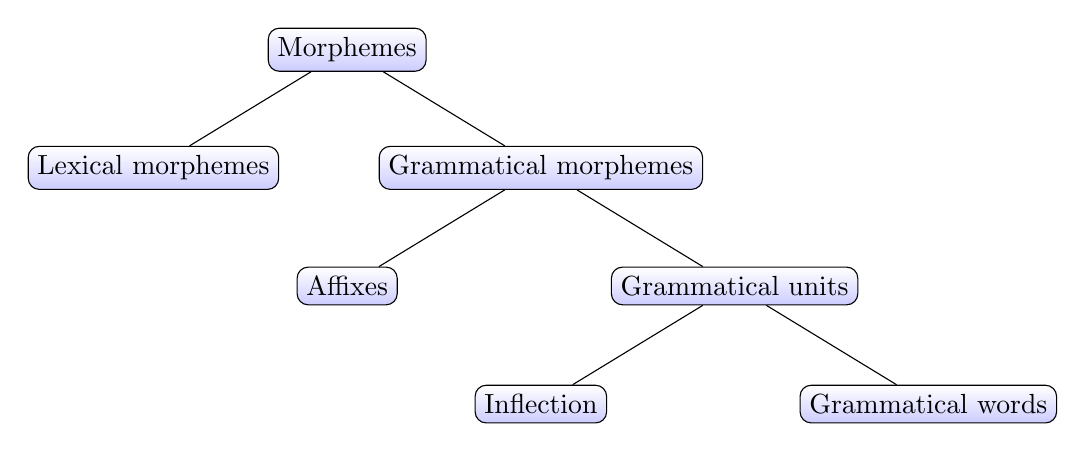
\begin{tikzpicture}[sibling distance=14em,
			every node/.style = {shape=rectangle, rounded corners,
					draw, align=center,
					top color=white, bottom color=blue!20}]]
		\node {Morphemes}
		child { node {Lexical morphemes} }
		child { node {Grammatical morphemes}
				child { node {Affixes} }
				child { node {Grammatical units}
						child { node {Inflection} }
						child { node {Grammatical words} }
					}};
	\end{tikzpicture}
\end{figure}

There are three main aspects in NLP morphological analysis :
\begin{enumerate}
	\item Lemmatization \& Stemming
	\item PoS tagging
	\item Disambiguation
\end{enumerate}

\paragraph{Lemmatization \& Stemming}

\begin{itemize}
	\item \textbf{Lemmatization \& Stemming :} ``The goal of both stemming and lemmatization is to reduce inflectional forms and sometimes derivationnaly related forms of a word to a common base form''. :
	      \begin{itemize}
		      \item \textbf{Stemmers :} A heuristic process, often used in information retrieval, that chops off the ends of words to produce word stems (engineer approach).
		      \item \textbf{Lemmatization :} based on Morphological dictionaries and morphological analysers (linguistic approach)
		      \item \textbf{Morphological dictionnaries.}
	      \end{itemize}

	      \begin{tabular}{|p{0.9\textwidth}|}
		      \hline
		      \textbf{Porter Algorithm :} Definitions
		      \begin{itemize}
			      \item $v \in $ $\lbrace$ A, E, I, O, U, Y iff C+Y $\rbrace$
			      \item $c \in $ $\lbrace$ alphabet-$v$ $\rbrace$
			      \item $V$ a sequence of $n$ $v$, $n>0$
			      \item $C$ a sequence of $n$ $c$, $n>0$
			      \item word $\in \lbrace[C](VC)^{\lbrace m\rbrace} [V] ~ | ~ [C], [V], m \geq 0 \rbrace$ where [C] and [V] $\ge$ 0 and (VC) can be repeated m times
		      \end{itemize}
		      \\
		      Algorithm to remove a suffix : $(condition\ on\ stem)S1 \rightarrow S2;$ if the condition is true, then a replacement can occur. Try each rules and make 5 successive run of the algorithm. \\
		      \textbf{Porter Algorithm :} Rule and condition example
		      
			  \noindent Rule : S1 $\rightarrow$ S2
		      \ex{ ($m$ > 1) EMENT $\rightarrow$ $\emptyset$;
		      REPLACEMENT $\rightarrow$ REPLAC;
		      DEMENT $\rightarrow$ DEMENT}\\
		      \\
		      Five successive runs, one of the rule match next run starts. \\
		      \hline
	      \end{tabular}

	      \medskip

	\item \textbf{under-stemming error :} Algo failed to group two words sharing conceptual meaning.
	\item \textbf{over-stemming error :} Algo grouped words having no shared conceptual meaning.
\end{itemize}

\medskip

\section{Corpus processing and analysis}

\subsection{Corpus}
\begin{itemize}
	\item \textbf{Corpus :} A large body of linguistic evidence typically composed of attested language use : Eveyrday conversations, radio news broadcasts, published writing, ...
	      \begin{itemize}
		      \item Machine readable
		      \item Sampled (aiming at balance representativeness), because it is impossible to collect all occurences of a language
		      \item well-organized and formatted
		      \item Big is beautiful
	      \end{itemize}
\end{itemize}

\subsubsection{Types and collection}
\begin{itemize}
	\item \textbf{Monolingual :}
	      \begin{itemize}
		      \item \textbf{Reference corpus :} large, balanced and ``representative''; designed to provide a comprehensive information about a language.
		      \item \textbf{Specialized corpus :} designed to cover one particular aspect of the language
		      \item \textbf{Monitor corpus :} (as opposed to a \textbf{static}) corpus with new materials
	      \end{itemize}
	\item \textbf{Multilingual :}
	      \begin{itemize}
		      \item \textbf{Comparable corpora :} collection of corpus of various languages with the same sampling method and similar balance to permit comparisons between corpora.
		      \item \textbf{Parallel corpora :} corpus in one language and its translation in conjunction with alignement techniques.
	      \end{itemize}
\end{itemize}

\subsection{Corpus annotation}
\begin{itemize}
	\item Aiming to make explicit some linguistic information that is part of the text $\rightarrow$ Adding metadata.
	      \begin{itemize}
		      \item Annotation : improve corpora usability
		      \item access deeper linguistic levels not accessible on the surface of the text.
	      \end{itemize}
	\item Automatic or manual.
	\item Levels :
	      \begin{enumerate}
		      \item Orthographic annotation (markup, italics, ...)
		      \item Phonetic/phonemic annotation (transcription of speech sounds)
		      \item Prosodic annotation (syllables, intonation contours) \ex{\lstinline{\*^w=ell\#}}
		      \item Morpho-syntactic annotation (part of speech, grammatical tagging) \ex{Origin/NN of/IN state/NN automobile/NN}
		      \item Syntactic annotation
		      \item Semantic annotation
		      \item Discoursal annotation (when a pronoun refers to something that has been said before).
	      \end{enumerate}

	      %
	      %\item There exists Standards of annotation
	      %\begin{itemize}
	      %\item corpora reusability and software interoperability
	      %\item langage resources dev. is expensive and time-consuming
	      %\item preserve language resources over time.
	      %\item $\rightarrow$ XML \& Unicode
	      %\item $\rightarrow$ Metadata
	      %\item $\rightarrow$ International standards.
	      %\end{itemize}
	      %For example : TEI.
\end{itemize}


\subsection{Corpus tokenization}
\begin{itemize}
  \item \textbf{token} : an instance of a sequence of characters in some particular document that are grouped together as a useful semantic unit for processing
  \item \textbf{type} : the class of all tokens containing the same character sequence
  \item \textbf{difficulties} : some languages don't uses spaces like us, or don't even have an alphabet; detection of the end of sentence \ex{Dr. Stone lives here.}
\end{itemize}


\newpage
\section{N-grams}
\begin{itemize}
	\item \textbf{Count histograms :}
	      \begin{itemize}
		      \item Few events appear very frequently
		      \item Most events appear only a few times
		      \item Many possible events never appear
		      \item \textbf{Zipf's Law :}
		      
		            \begin{minipage}{.45\textwidth}
                        Specific distribution, Linear in log-log scale defines power law :
                        $$
                          \begin{array}{ccc}
                              \log y & = & -a\cdot\log x + \log b \\
                              \log y & = & \log (bx^{-a})         \\
                              y      & = & bx^{-a}                \\
                          \end{array}
                        $$
		            \end{minipage}\hfill
		            \begin{minipage}{.45\textwidth}
			            \center\includegraphics[width=0.95\linewidth]{images/zipf.png}
		            \end{minipage}
	      \end{itemize}
	\item \textbf{N-Gram Probability :} The \emph{conditional probability} of observing a word $w$ at a position $i$ given a \emph{history} $h = w_{i-n+1} \dots w_{i-2}w_{i-1}$ (or \emph{N-gram context}) of preceding words :
	      $$P(X_i = w_i | X_{i-n+1} = w_{i-n+1}, \dots, X_{i-2} = w_{i-2}, X_{i-1} = w_{i-1}) \overset{notation}{=} P(w_i|h)$$
	      \begin{itemize}
		      \item Random variables $X_i, X_{i-1}, X_{i-2}, ...$ are implicit in the shorter notation and take their value in a fixed vocabulary : $w_i \in W, \forall i$.
		      \item The model is assumed stationary : it does not depend on the position $i$ in the text : $P(w_i | h) = P(w|h), \forall i$.
		      \item The history $h$ for a N-gram is made of the $N-1$ preceding words.
		      \item The word $w$ is said to be predicted given a known history $h$.
	      \end{itemize}
\end{itemize}

We can generalize this probability to a sentence probability, using chain rule and N-gram assumption, we have for a sentence of $n$ words :
\begin{eqnarray*}
	P(w_1 \dots w_n) &=& P(w_1^n) = P\left(w_{1}\right) P\left(w_{2} \mid w_{1}\right) P\left(w_{3} \mid w_{1}^{2}\right) \ldots P\left(w_{n} \mid w_{1}^{n-1}\right)\\
	&=& \prod^n_{k=1} P(w_k|w_1^{k-1})\\
	&\approx & \prod^n_{k=1} P(w_k|w_{k-N+1}^{k-1})\\
	&=& P\left(w_{1}\right) P\left(w_{2} \mid w_{1}\right) P\left(w_{3} \mid w_{1} w_{2}\right) \underbrace{P\left(w_{4} \mid w_{2} w_{3}\right) \ldots P\left(w_{n} \mid w_{n-2} w_{n-1}\right)}_{approximation,\ we\ only\ take\ n\ preceding\ words}
\end{eqnarray*}

\subsection{Estimation}
\begin{itemize}
	\item \textbf{Maximum likelihood estimation} :
	      \medskip

	      \begin{tabular}{|p{0.9\textwidth}|}
		      \hline
		      \textbf{Maximum likelihood}
		      $$\hat{P}(w|h) = \left\lbrace
		      \begin{array}{cl}
				      \frac{C(h,w)}{C(h)} & if\ C(h) > 0 \\
				      0                   & otherwise   \\
			      \end{array}\right.$$
		      \begin{itemize}
			      \item $C(h,w)$ the number of times the history $h$ is followed by $w$ in the training corpus;
			      \item $C(h)$ the number of times the history $h$ is observed in the training corpus.
		      \end{itemize}
		      \\
		      \textbf{Consistency property}
		      $$\forall h ~~, ~~ \sum_{w\in W} P(w|h) = 1$$
		      \\
		      \hline
	      \end{tabular}
	\item For a 1-gram, the history $h$ is empty so $C(h)$ becomes $C(h) = M$, and $C(h,w) = C(w)$. $M$ is the total number of word tokens in the training corpus (= the corpus length). It's different to $W$ which is the vocabulary size, so the number of different words in the corpus. Formulated differently: $M = len(L)\ and\ \mid W\mid = len(set(L))$
	\item Need smoothing because observed events are overestimated and other possible events have a zero probability.
	\item Smoothing techniques are required to correct the MaxLikelihood  estimation and the consistency property still need to be satisfied !
\end{itemize}

\subsection{Smoothed N-grams}
\begin{itemize}
	\item \textbf{Pseudo-counts and Laplace Smoothing :}

	      \medskip

	      \begin{tabular}{|p{0.9\textwidth}|}
		      \hline
		      \textbf{Bayesian estimation}

		      Define a priori pseudo-counts $C^*(h,w)>0$ for any possible events
		      $$\hat{P}(w|h) = \frac{C(h,w)+ {\color{red} C^*(h,w)}}{C(h)+ {\color{red}  \sum_{w}C^*(h,w)} }$$
		      The red part is new and is called the prior probability.\\
		      \textbf{Laplace smoothing}

		      Set $C^*(h,w) = 1$ for all events $\rightarrow$ uniform priors and $\sum_{w}C^*(h,w) = |W|$ \\
		      \hline
	      \end{tabular}

	      \medskip

	\item \textbf{Linear Interpolation :}

	      \medskip

	      \begin{tabular}{|p{0.9\textwidth}|}
		      \hline
		      \textbf{Linear Interpolation}

		      Build estimators for \emph{several model orders} $\rightarrow$ vary history length and combine them linearly :
		      $$\hat{P}(w|h) = \lambda_0 \hat{P}_{ML}(w|h) + \lambda_1 \hat{P}_{ML}(w|h_{-1}) + \dots + \lambda_p \hat{P}_{ML}(w|h_{-p}) $$
		      where $h = X_{i-N+1}\dots X_{i-1} $ (N gram history)\\
		      $h = X_{i-N+2}\dots X_{i-1}$ (N-1 gram history). ``i'' represent our ``advancement'' in the history.\vspace{\baselineskip}
		      
		      \textbf{Mixture Model}

		      In a general case we can combine $k$ estimators :
		      $$ \hat{P}(w|h) = \sum_{i=1}^k \lambda_i \hat{P}_i(w|h) ~~ \mathrm{with} ~~ \sum_{i=1}^k \lambda_i = 1$$
		      \\
		      \textbf{EM estimation of $\lambda$ 's (EM=estimation maximisation)}

		      A validation corpus $S=\lbrace w_1, \dots, w_M\rbrace$ (here and only here: M is the size of S)
		      \begin{itemize}
			      \item Initialize : $\lambda_i = \frac{1}{k}, ~~ \forall considered\ i$
			      \item E-step : $E(Model_i|S) = \sum_{j=1}^M \frac{\lambda_i \hat{P}_i(w_j|h)}{ \sum_{l=1}^k \lambda_i \hat{P}_l(w_j|h)}$
			      \item M-step : $\lambda_i = \frac{E(Model_i|S)}{M}$
		      \end{itemize}                                                                                  \\
		      \hline
	      \end{tabular}

	      \medskip

	\item \textbf{Backoff Smoothing :}

	      \medskip

	      \begin{tabular}{|p{0.9\textwidth}|}
		      \hline
		      \textbf{Backoff Smoothing}
		      $$ \hat{P}(w|h) = \left\lbrace \begin{array}{lcl}
				      max\left(0, \frac{C(h,w) - d_c}{C(h)} \right) + \gamma(h)\hat{P}_{back}(w|h) & if & C(h) > 0 \\
				      \hat{P}_{back}(w|h)                                      & if & C(h) = 0                   \\
			      \end{array}\right. $$
		      with :
		      \begin{itemize}
			      \item $\gamma (h) = \sum_{w:C(h,w)>0} \frac{d_c}{C(h)}$ = the total discounted probability mass distributed over unobserved N-grams
			      \item distributed over seen and unseen events (Katz version only  over unseen events)
			      \item proportionally to a back-off distribution $\hat{P}_{back} = \hat{P}(w|h_{-1})$ (in the simplest case) 
			      \item $\hat{P}_{back}$  is smoothed using the same formula recursively but not with the same counts. The recursion stops on 1-gram: $\hat{P}(w) = \frac{C(w)}{M}$ or on ``0-gram'' $\hat{P}(w) = \frac{1}{\mid W\mid}$  with M=\# tokens in training and $\mid W\mid$ = vocabulary size.
		      \end{itemize} \\
		      
		      \textbf{Discounting parameter}
		      $$d_c \overset{\Delta}{=} d, ~~ \forall c $$
		      Estimation of an upper bound $d_{*}$ with $n_c$, the number of N-grams occurring $c$ times :
		      $$d\leq d_{*} = \frac{n_1}{n_1+2 n_2}$$
		      most practical cases : $n_1, n_2 > 0 \rightarrow 0 < d < 1$\vspace{\baselineskip}
		      
		      Other technique: Good Turing
		      $$C - d_c = (C + 1) \dfrac{n_{C+1}}{n_C}$$\\
		      Good-Turing discounting can be limited to small counts as the counts decreases a lot for small grams, but not really for bigger grams.\\ 
		      
		      \textbf{Backoff Smoothing improved: Kneser-Ney modified counts:}\\
		      Same formula but with $\hat{P}_{back} = \frac{C^{*}\left(h_{-1}, w\right)-d_{C}}{\sum_{w^{\prime}} C^{*}\left(h_{-1}, w^{\prime}\right)}$ with $C^*(h_{-1}, w)$ the number of different shorter histories $h_{-1}$  where the word $w$ has been observed, ignoring the frequency of these events. It's then counting how many \emph{different} words follows the history, without looking how many times a word is used after the history.\\
		      
		      If we have C(like computers) = 5, C(buy computers) = 3, C(sell computers) = 4 $\Rightarrow C^*(h_{-1}, computers) = 3$, and $C^* (h_{-1}, apples) = 1$ and $C^* (h_{-1}, books) = 2$; we would have counted $\hat P_{back} = \frac{5+3+4}{1+2+3+4+5}$ before. Now we have $\hat P_{back}^*(w\mid h) = \frac{3}{1+2+3}$.\\
		      
		      \hline
	      \end{tabular}

\end{itemize}

\subsection{Performance assessment}
\begin{itemize}
	\item \textbf{Basic Protocol :} Split available data into training (90\%, model) and test (10\%, evaluate) sets.
	\item \textbf{Refinement 1 :} Training set into 90\% actual training and 10\% held-out to tune \emph{meta-parameters} and select optimal model order.
	\item \textbf{Refinement 2 :} 10-fold cross-validation
	\item \textbf{Test set perplexity}

	      \medskip

	      \begin{tabular}{|p{0.9\textwidth}|}
		      \hline                                                                \\
		      \textbf{Per-symbol Log Likelihood $LL$ :} here M is the size of the test set = the number of words to predict.
		      $$ LL = \frac{1}{M} log(\prod_{i=0}^M P(w_i \mid h))= \frac{1}{M} \sum_{i=1}^M \log P(w_i|h) $$
		      \\
		      \textbf{Test set perplexity $PP$}
		      $$ PP = 2^{-LL}$$
		      The lower, the better, valid measure only if \emph{consistent model} !
		      \\
		      \hline
	      \end{tabular}

	      \medskip

	\item \textbf{Test set perplexity properties}
	      \begin{itemize}
		      \item When playing shannon game : Perplexity is an average weighted branching factor when guessing the next word :
		            \begin{eqnarray*}
			            PP &=& 2^{\left[ - \frac{1}{M} \sum_{i=1}^M \log P(w_i|h) \right]}\\
			            &=& 2^{\left[ \log \prod_{i=1}^M P(w_i|h)^{- \frac{1}{M}} \right]}\\
			            &=& \sqrt[M]{\prod_{i=1}^M \frac{1}{P(w_i|h)}}\\
		            \end{eqnarray*}
		      \item With 0-gram : $$PP = \sqrt[M]{\prod_{i=1}^M \frac{1}{P(w_i|h)}} = \sqrt[M]{|W|^M} = |W|$$ When we use 0-grams, we predict uniformly at random.
		      \item \emph{Better models} have a \emph{lower perplexity} (more predictive)
		      \item Unsmoothed models have $\exists i, P(w_i|h) = 0 \rightarrow PP = +\infty$ worst than random.
		      \item Start of sentence ($<s>$) is never predicted, end ($</s>$) is predicted, the actual number of predictions in a test set of $k$ sentences of $n_k$ words is $M = \sum^k_{j=1} (n_k + 1)$ there is a $+1$ for th $</s>$ in this formula.
		      \item Training set PP decreases with model order so you must avoid \emph{overfitting}, Test set PP is minimal for an optimal order (often 3-gram)
	      \end{itemize}

	\item \textbf{Unknown words}
	      \begin{itemize}
		      \item The vocabulary $W$ may not contain all the words of the test set, representative of new data;
		      \item A consistent model assign a zero probability to any new word $\rightarrow PP = + \infty$
		      \item Define an additional word type : UNK as part of the vocabulary and relies on smoothing : Either from some out-of-vocabulary (OOV) words, or purely from smoothing mechanism $C(h,<UNK>)$ or with interpolation or backoff to a zero-gram $P(<UNK>)= \frac{1}{\mid W \mid}$.
	      \end{itemize}
	
	\item \textbf{Remark :}
        The fewer training data we haven the better the smoothing ought to be! $\rightarrow$ Increasing the model order may result in less predictive models if the smoothing is poor
\end{itemize}

\section{HMM}
\subsection{PoS Tagging}
\label{PoSHMM}
\begin{itemize}
	\item \textbf{Observation}
	      \begin{itemize}
		      \item Tagging is \emph{ambiguous}, a probabilistic approach relies on the frequencies of word-tag associations in a training corpus to assign the tag of each word in a \emph{new sentence}.
		      \item Choose most likely tag $\rightarrow$ always same tag for a same word :/
		      \item Choose tag according to its context $\rightarrow$ HMM.
		      \item word sequence is observed, tag sequence is hidden $\rightarrow$ HMM.
	      \end{itemize}
	\item \textbf{Probabilistic finite state model}
	      \begin{itemize}
		      \item Each state $\rightarrow$ PoS tag
		      \item Each state $\rightarrow$ emits words according to emission probability distribution
		      \item State sequence is hidden, emitted words is observed
		      \item Find the most likely state sequence given the observed word sequence $\rightarrow$ global criterion to tag words (as it looks at the whole sentence at one go).
	      \end{itemize}
\end{itemize}

% \subsection{From Markov chains to HMMs}
% \begin{itemize}
% 	\item \textbf{$p$-order Markov Chain} :
% 	      \begin{itemize}
% 		      \item A discrete time finite Markov Chain is a stochastic process $\lbrace X_t|t\in \mathbb{N}\rbrace$ where the random var $X$ takes its value at any discrete time $t$ in a finite set $W$ and such that : $$ P(X_t = w | X_0, \dots, X_{t-2}, X_{t-1}) = P(X_t = w | X_{t-p}, \dots, X_{t-1}) \overset{\Delta}{=} P(w|h)$$
% 		            with a markov chain order $p$, a $N$-gram with $N = p+1$.
% 	      \end{itemize}
% 	\item \textbf{Standard cases :}
% 	      \begin{itemize}
% 		      \item Order 1 : only previous event
% 		      \item Stationary : MC does not depend on t :

% 		            \medskip

% 		            \begin{tabular}{|p{0.8\textwidth}|}
% 			            \hline                                                                        \\
% 			            \textbf{Transition matrix and Initial Probability}

% 			            A stationary finite order 1 MC is characterized by a \emph{transition matrix}
% 			            $$ P = [p_{ij}] = [P(X_t = w_j|X_{t-1} = w_i)]$$
% 			            and an \emph{initial probability} vector $\pi^0$ :
% 			            $$\pi^0 = P(X_0 = w_i)$$
% 			            \\
% 			            \hline
% 		            \end{tabular}
% 	      \end{itemize}

% 	      \medskip

% 	\item \textbf{Finite State Representation} : For order 1, each state represents one word, and use $W$ as a set of state, $P$ the transition prob and $\pi^0$ the initial prob. For order 2, extend the state space : $W^2$, states emits a single word but the transition probabilities depends on the last two words. The maximal number of states of a MC of order $p$ is $|W|^p$ and grows exponentially with $p$.

% 	\item \textbf{No finite order} : Some finite state machines model a broader class of distributions.
% 	\item \textbf{Not reducible :} A model not reducible to a finite order MC : for any finite window (history) length, there exists some ambiguous strings. This richer class is actually a special case of HMM.

% 	\item \textbf{Sentence probability}

% 	      \medskip

% 	      \begin{tabular}{|p{0.9\textwidth}|}
% 		      \hline
% 		      \\
% 		      \textbf{Sentence probability}

% 		      The probability of a sentence $s = w_0 \dots w_{|s|-1}$, also called \emph{likelihood} $P(s|M)$ of $s$ according to a first order Markov Chain $M$ :
% 		      $$P(s|M) = \prod_{i=0}^{|s|-1} P(w_i|M) = P(X_0 = w_0) \prod_{i=1}^{|s|-1} P(X_i = w_i | X_{i-1} = w_{i-1}) = \pi^0 \prod_{i=1}^{|s|-1} P_{w_{i-1}w_{i}}$$ \\
% 		      \hline
% 	      \end{tabular}

% 	      \medskip

% \end{itemize}

\subsection{HMM definition}
\begin{itemize}
	\item
	      \begin{tabular}{|p{0.9\textwidth}|}
		      \hline
		      \\
		      \textbf{Hidden Markov Models :} Definition

		      A discrete HMM with state emission :
		      \begin{itemize}
			      \item $W$ is a finite \emph{vocabulary}
			      \item $Q$ is a set of \emph{states}
			      \item $A$ is a $|Q|\times |Q|$ \emph{transition probability} matrix ($\sum_{q'\in Q} A_{qq'} = 1, ~\forall q\in Q$) $\rightarrow$ sum of \emph{outgoing} transitions = 1
			      \item $B$ is a $|Q|\times |W|$ \emph{emission probability} matrix ($\sum_{w\in W} A_{qw} = 1, ~\forall q\in Q$)
			      \item $\pi$ an \emph{initial probability} distribution vector ($\sum_{q\in Q} \pi_q = 1$)
		      \end{itemize} \\
		      \hline
	      \end{tabular}

	      \medskip

% 	\item \textbf{Discrete Hidden Markov Models :} Markov Chains ?
% 	      \begin{itemize}
% 		      \item $W$ and $Q$ may have distinct cardinalities
% 		      \item Transition probability matrix become $A$ instead of $P$, emission probability matrix contains additional parameters
% 		      \item A string is not necessarily generated along a single state sequence
% 		      \item States are hidden and HMMs define larger class of distributions.
% 	      \end{itemize}

	\item \textbf{Likelihood}

	      \medskip

	      \begin{tabular}{|p{0.9\textwidth}|}
		      \hline

		      \textbf{Path likelihood :}

		      The likelihood $P(s,\nu |M)$ of a sequence $s = s_1 \dots s_{|s|}$ along a path or a state sequence $\nu = q_1 \dots q_{|s|}$ in a HMM $M$ :
		      $$P(s,\nu |M) = \prod_{i=1}^{|s|} P(s_i,q_i|M) = \pi_{q_1} B_{q_1s_1} \prod_{i=2}^{|s|} A_{q_{i-1}q_i} B_{q_is_i} $$
		      Example: $P(abb, 122|M) = 0.4 \times 0.2 \times 0.9 \times 0.1 \times 0.3 \times 0.1$
		      
		      Interpretation: Probability to observe the sentence a b b generated by the sequence of POStags 1 2 2
		      
		      {\centering
		      \includegraphics[width=.3\linewidth]{images/path-likelihood.png}\par
		      }
		      \\
		      \textbf{Sequence likelihood}

		      The likelihood $P(s|M)$ of a sequence $s = s_1 \dots s_{|s|}$ in a HMM $M$ is :
		      $$P(s|M) = \sum_{\nu\in Q^{|s|}} P(s,\nu |M)$$
		      Example: $P(abb|M) = P(abb, 111|M) + P(abb, 112|M) + P(abb, 121|M)+P(abb, 122|M) + P(abb, 211|M) +\dots$
		      
		      Interpretation: Probability to observe the sentence a b b generated by \emph{any} sequence of 3 POStags
		      
		      Note : $\mathcal{O}(|Q|^{|s|})$ possible state sequences \\
		      \hline
	      \end{tabular}

\end{itemize}

\subsection{HMM Fundamental questions}\label{fundamental}
\begin{itemize}
	\item \textbf{Viterbi decoding} Given a sentence (= sequence of words assumed to have been produced by a HMM) which is the most likely state sequence of POStags that produced it?
	      $$\nu^{*} = \arg\max_{\nu} P(s, \nu |M)$$
	\item \textbf{Viterbi recurrence}
	
	        Most likely state sequence for abb = 212:
	        
	      {\centering
	      \includegraphics[width=.4\linewidth]{images/viterbi.png}
	      \par}
	      
	      We propagate the probabilities among the nodes (states). Every nodes remembers which node as the local highest probability pointing to him. When all nodes are crossed, back-propagate following the maximum of each node.

	      \begin{tabular}{|p{0.9\textwidth}|}
		      \hline
		      \textbf{Viterbi recurrence}

		      \emph{Auxiliary quantity} : $\gamma (k,t) = P(s_1 \dots <_t, \nu_t^{*} = k | M)$ : The probability that the most likely path $\nu^{*}$ reaching state $k$ at step $t$.

		      \begin{itemize}
			      \item Initialize : $\gamma (k,1) = \pi_k B_{k,s_1} \forall k$
			      \item Recurrence : $\left\lbrace \begin{array}{lcl}
					            \gamma (k,t) & = & \max_{l}(\gamma(l,t-1)A_{lk}) B_{ks_t} \\
					            back(k,t)    & = & \arg\max_{l}(\gamma(l,t-1)A_{lk})      \\\end{array}\right.$
			      \item Termination : $\left\lbrace \begin{array}{lcl}
					            P(s,\nu^{*} |M) & = & \max_l \gamma (l, |s|)     \\
					            q_{|s|}^{*}     & = & \arg\max_l \gamma (l, |s|) \\\end{array}\right.$
		      \end{itemize}
		      \\
		      \hline
	      \end{tabular}

	      \medskip

	\item \textbf{Viterbi alignment :}
	      \begin{itemize}
		      \item $P(s, \nu^{*})$ gives the probability of an optimal path $\nu^{*}$
		      \item Computations are done usually with log's : $$ -\log \gamma (k,t) = \min_{l}(-\log \gamma(l,t-1) - \log A_{lk}) - \log B_{ks_t} $$
		      \item $back$ is a backpointer to recover the actual path $\nu^{*}$
		      \item Time complexity : $\Theta (m\times |s|)$ with $m$ the number of transitions
		      \item The path $\nu^{*}$ defines an \emph{alignment} between states and words
		      \item This \emph{alignement} defines a \emph{segmentation} of the sequence.
	      \end{itemize}

% 	\item \textbf{Forward recurrence :}
% 	      \medskip

% 	      \begin{tabular}{|p{0.9\textwidth}|}
% 		      \hline
% 		      \textbf{Forward recurrence}

% 		      \emph{Auxiliary quantity} : $\alpha (k,t) = P(s_1 \dots <_t, \nu_t = k | M)$ : The likelihood of emitting the first $t$ words and reeaching state $k$ at time $t$.

% 		      \begin{itemize}
% 			      \item Initialize : $\gamma (k,1) = \pi_k B_{k,s_1} \forall k$
% 			      \item Recurrence : $\gamma (k,t) = \sum_{l}(\alpha(l,t-1)A_{lk}) B_{ks_t}$
% 			      \item Termination : $P(s,\nu^{*} |M) = \sum_l \alpha (l, |s|)$
% 		      \end{itemize}

% 		      Same time complexity : $\Theta (m|s|)$ \\
% 		      \hline
% 	      \end{tabular}

% 	      \medskip
    
	\item \textbf{Learning problem :} Given an HMM structure (by default, a fully connected graph) and several sentences (a training corpus) to model, estimate the HMM parameters : $A, B, \pi$

	\item \textbf{Supervised learning :} The learning sentences are annotated with their respective states :

	      \begin{tabular}{|p{0.9\textwidth}|}
		      \hline
		      \begin{itemize}
			      \item $B_{ki} = \hat P(w_i|k) = \frac{C(k,w_i)}{C(k)}$
			            \begin{itemize}
				            \item $C(k,w_i)$ the number of times words $w_i$ is observed on state $k$
				            \item $C(k)$ the number of times the state $k$ is used
			            \end{itemize}
			      \item $A_{kl} = \hat P(l|k) = \frac{C(k,l)}{C(k)}$
			            \begin{itemize}
				            \item $C(k,l)$ the number of times a transition from state $k$ to state $l$ occur.
			            \end{itemize}
			      \item $\pi_k = \frac{C_1(k)}{\sum^{|Q|}_{j=1}C_1(j)}$
			            \begin{itemize}
				            \item $C_1(k)$ the number of times the state $k$ is used as first state
			            \end{itemize}
		      \end{itemize}\\
		      Note: A and B can be smoothed.
		      \\
		      \hline
	      \end{tabular}

	      \medskip

% 	\item \textbf{Viterbi training :} unsupervised learning : The training corpus is made of un-annoted sentences. The mapping between states (=PoS tags) and observations (=words) is \emph{a priori} unknown :

% 	      \medskip

% 	      \begin{tabular}{|p{0.9\textwidth}|}
% 		      \hline
% 		      \begin{enumerate}
% 			      \item Fix initial parameters values $A^0, B^0, \pi^0$
% 			      \item Repeat
% 			            \begin{enumerate}
% 				            \item Compute a most likely path through a Viterbi alignment for each training sentence given the parameters $A^i, B^i, \pi^i$
% 				            \item Estimate the emission and transition frequencies from such paths
% 				            \item Recompute the parameter values $A^{i+1}, B^{i+1}, \pi^{i+1}$ from those frequenties
% 			            \end{enumerate}
% 			            till some stopping criterion is met (max iter)
% 		      \end{enumerate}
% 		      \\\hline
% 	      \end{tabular}

% 	      \medskip

	\item \textbf{Forward-Backward or Baum-Welch Algorithm :} Unsupervised algorithm
	      \begin{itemize}
		      \item Viterbi training is an approximation as it considers that each training sentence is generated along a single path (a most likely one).
		      \item A more accurate estimation is obtained if one considers all possible paths to generate each sentence : Actual frequencies are replaced by expected frequencies, it's a special case of EM procedure.
		      \item Viterbi and Baum-Welch training are both sensitive to parameter initialization.
	      \end{itemize}
\end{itemize}

\section{PoS Tagging}

\begin{itemize}
	\item \textbf{The sequence labelling problem :} We have to associate a PoS tag to each word token in a sentence.
	\item \textbf{Tagsets :} There exist different tagset, for example : 45-tag Penn TreeBank or 87-tag Brown Corpus tagset.
	      \begin{itemize}
		      \item Despite having coarser tags, the 45-tag Treebank tagset is more ambiguous (a same word have several tags).
		      \item It's however most commonly used at least for evaluating automatic taggers
	      \end{itemize}
\end{itemize}

\subsection{Approaches}
\begin{itemize}
	\item \textbf{Rule-based approach}
	      \begin{enumerate}
		      \item Use a large dictionary to assign each word a set of possible tags
		      \item Apply a large list of \emph{disambiguation rules} to restrict each set to a single tag for each word.
	      \end{enumerate}

	\item Limitations of the rule-based approach :
	      \begin{itemize}
		      \item Dictionary and disambiguation rules are specific to a given language
		      \item Those linguistic resources need to be constantly updated while language evolves :/
	      \end{itemize}

	\item \textbf{Probabilistic approach}
	      \begin{itemize}
		      \item Considering \ref{PoSHMM} : A better probabilistic model assigns a tag to a word according to its context : HMM PoS-tagging :
		            \begin{itemize}
			            \item words = observation discrete emission probabilities
			            \item tag = specific state
			            \item tagging reduces to find the most likely state sequence = \emph{Viterbi decoding}
		            \end{itemize}
	      \end{itemize}

	\item \textbf{Transformation-based tagging :}

	      \begin{itemize}
		      \item Like rule-based approaches, each word is tagged according to some \emph{explicit rules}
		      \item Like probabilistic approaches, a disambiguation model is learned from a corpus of tagged sentences (supervised learning)
		            \medskip

		            \begin{tabular}{|p{0.9\textwidth}|}
			            \hline
			            \\
			            \textbf{Brill tagger :} Definition
			            \begin{enumerate}
				            \item The most likely tag is first assigned to each word
				            \item Change the current tag by applying an ordered list of \emph{transformation rules}
				            \ex{Change NN to VB when the previous tag is TO}
			            \end{enumerate}
			            \\
			            \textbf{Learning Transformation Rules :}

			            Given a PoS tagged corpus and \emph{transformation templates} such as : Change tag \textbf{a} to \textbf{b} when :
			            \begin{itemize}
				            \item the preceding/following word is tagged \textbf{z}
				            \item the word two before/after is tagged \textbf{z}
				            \item the preceding/following word is tagged \textbf{z} and the word two before/after is tagged \textbf{w}
			            \end{itemize}

			            \begin{algorithmic}
				            \REQUIRE A tagged corpus, some templates of rule, a vocabulary
				            \ENSURE An ordered list of transformation rules
				            \STATE Tag each word with its most likely tag
				            \REPEAT
				            \STATE Try every possible transformation by instantiating some template
				            \STATE Select the one that results in the most improved tagging
				            \STATE Relabel the corpus accordingly
				            \UNTIL{\emph{stopping criterion is met;} $\rightarrow$ ex: when no progress is made anymore.}
			            \end{algorithmic}
			            \\
			            \hline
		            \end{tabular}

		            \medskip

		      \item Pros :
		            \begin{itemize}
			            \item Transformation rules can be easily interpreted linguistically
			            \item Learning those rules makes it possible to adapt the tagger to several languages (or language evolutions)
		            \end{itemize}
		      \item Limitations :
		            \begin{itemize}
			            \item A transformation rule can be learned only if it is an instance of abstract transformation template
			            \item Learning is \emph{supervised} only $\rightarrow$ a tagged corpus is mandatory
			            \item Computational complexity of learning is an issue.
		            \end{itemize}
	      \end{itemize}
\end{itemize}

\subsection{HMM PoS tagging}
\begin{itemize}
	\item \textbf{First-order Markov Chain Structure}
	      \begin{itemize}
		      \item This is equivalent to a TAG Bigram model as it is guessing the next state knowing the current state.
		      \item Such a model can be estimated from a tagged corpus $\rightarrow$ counting the successive POS tags $transition\ probability = \hat P(VB|TO) = \dfrac{C(TO,BV)}{TO}$.
		      \item However TAGs are not observed when a new sentence need to be tagged.
	      \end{itemize}
	\item \textbf{HMM tagger :}
	      \begin{itemize}
		      \item first-order MC: transition probabilities
		      \item emission probabilities
	      \end{itemize}
	\item \textbf{HMM Tagging = Viterbi decoding}
	      \medskip

	      \begin{tabular}{|p{0.9\textwidth}|}
		      \hline                                                                                                                                                         \\
		      Given a sequence of $n$ words $w_1^n = w_1, \dots, w_n$ find a sequence of $n$ tags $\hat{t}^n_1$ that maximises the posterior probability (MAP decision rule)
		      \begin{eqnarray*}
			      \hat{t}^n_1 &=& \arg\max_{t^n_1} P(t^n_1 | w^n_1)= \arg\max_{t^n_1} \underset{likelihood}{\underbrace{P(w^n_1 | t^n_1)}} \underset{prior}{\underbrace{P(t^n_1)}}\\
			      &\approx & \arg\max_{t^n_1} \underset{Hyp. 1}{\underbrace{\prod^n_1 P(w_i | t_i)}} \underset{Hyp. 2}{\underbrace{\prod^n_1 P(t_i | t_{i-1})}}
			      = \arg\max_{t^n_1} \prod^n_1 \underset{Emission}{\underbrace{P(w_i | t_i)}} \underset{Transition}{\underbrace{P(t_i | t_{i-1})}}\\
		      \end{eqnarray*}
		      \begin{enumerate}
			      \item \emph{Hyp. 1 :} Each word $w_i$ given its tag $t_i$ is independent of the other words and tags
			      \item \emph{Hyp. 2 :} Bigram tag model
		      \end{enumerate}
		      \\
		      \hline
	      \end{tabular}

	      \medskip

	      \begin{itemize}
		      \item \textbf{Unsupervised learning}

		      \item Pro : fully automatic :
		            \begin{itemize}
			            \item Define a HMM strucuture with one state per tag in a tagset
			            \item Learn the HMM parameters $P(w_i | t_i)$ and $P(t_i | t_{i-1})$ using viterbi training or Baum-Welch on a text corpus (not tagged)
		            \end{itemize}
		      \item Limitations :
		            \begin{itemize}
			            \item Viterbi training and Baum-Welch are sensitive to initialization
			            \item The states are not necessarily associated with relevant tag set :
			                  \begin{itemize}
				                  \item Only the number of states is constrained by the number of tags
				                  \item Some linguistically informed post-processing needs to be done if one wants to map states to actual tags, whenever possible.
			                  \end{itemize}
		            \end{itemize}
	      \end{itemize}

	      \begin{itemize}
		      \item \textbf{Supervised learning} see section \ref{fundamental}'s ``Supervised learning'' paragraph for more details!

		            \medskip

		            \begin{tabular}{|p{0.8\textwidth}|}
			            \hline
			            \textbf{HMM supervised estimation}
			            \begin{itemize}
				            \item Copute counts from a training set of tagged sentences (sequence of Word/TAG pairs)
				            \item Build the probability estimates :
				                  $$\hat{P}(w_i|t_i) = \frac{C(t_i,w_i)}{C(t_i)} ~~~~ \hat{P}(t_i|t_{i-1}) = \frac{C(t_{i-1},t_i)}{C(t_{i-1})} $$
				            \item Smooth the probability estimates :
				                  \begin{itemize}
					                  \item Additive smoothing for emission probabilities :
					                        $$ \hat{P}(w_i|t_i) = \frac{C(t_i,w_i) + \epsilon}{C(t_i) + \sum_{w\in W} \epsilon} ~~~ 10^{-6} \leq \epsilon \leq 1 $$
					                  \item Possibly any bigram smoothing for transition probabilities.
				                  \end{itemize}
			            \end{itemize}
			            \\
			            \hline
		            \end{tabular}

		            \medskip

		      \item Pro :
		            \begin{itemize}
			            \item one can interpret the states as true PoS tags
			            \item no need to discover the meaning of the states after learning
		            \end{itemize}
		      \item Limitation :
		            \begin{itemize}
			            \item a tagged corpus is required in the first place
		            \end{itemize}
	      \end{itemize}

	\item \textbf{Tagging unknown word} :
	      $$ \hat{P}(w_i|t_i) = \frac{C(t_i,w_i) + \epsilon}{C(t_i) + \sum_{w\in W} \epsilon} ~~~ 10^{-6} \leq \epsilon \leq 1 $$

	      \begin{itemize}
		      \item \textbf{Problem :} Even with a smoothed emission probability, any OOV word in the set is assigned a zero probability, there is no Viterbi path, no path producing the observed sequence.
		      \item \textbf{Usual solution :}
		            \begin{itemize}
			            \item Replace any word occuring only once (hapax legomenon = singleton) in the training set with a UNK marker
			            \item Reduce the observed vocabulary accordingly and add UNK to it
			            \item Smooth the emission probability according to this new vocabulary
		            \end{itemize}
	      \end{itemize}
	\item \textbf{Extending HMM to Tag Trigrams}
	      \begin{itemize}
		      \item Given a sequence of $n$ words $w_1^n$ find a sequence of $n$ tags $\hat{t}^n_1$ :
		            $$ \hat{t}^n_1 \approx \arg\max_{t^n_1} \left[\prod_{i=1}^n P(w_i|t_i) P(t_i|t_{i-2}t_{i-1})\right] P(t_{n+1}|t_{n-1}t_{n}) $$
		      \item Viterbi decoding must be applied on an extended state space with one state per tag pairs $t_{i-2}t_{i-1}$ rather than one state per tag
		      \item Supervised learning is strongly recommended
		      \item Smoothing the tag trigram becomes an issue $\rightarrow$ apply classical N-gram smoothing methods


	      \end{itemize}
\end{itemize}

\subsection{Tagging performance}
\begin{itemize}
	\item Fill a \emph{confusion matrix}:
	
	Each row corresponds to an actual tag
	
	Each column corresponds to a predicted tag
	
	Each entry defines the error percentage with respect to an actual tag frequency $f(i)$
	
	\item Performance metrics :
	      \begin{itemize}
		      \item Average error rate per TAG : $\frac{1}{n_{rows}} \sum_i \sum_j error_{ij}$
		      \item Tagging error rate : $\frac{\sum_i f(i) (\sum_j error_{ij})}{\sum_i f(i)}$
		      \item Tagging accuracy = $100\%$ - Tagging error rate
	      \end{itemize}
\end{itemize}


\section{Machine Translation}
    \begin{tabular}{|p{0.9\textwidth}|}
    	\hline \\
    	\textbf{Machine Translation :} Problem definition \\
    	\emph{Machine Translation} concerns the use of computers to automate translation from a \emph{source language} to a \emph{target language} \\
    	\begin{center} \textit{``The process of translating comprises in its essence the whole secret of human understanding of the world and of social communication''}\end{center}
    	\begin{flushright} H.G. Gadamer, German Philosopher, 1900-2002\end{flushright} \\
    	\hline
    \end{tabular}
    
    \subsection{Difficulties}
    \begin{itemize}
    	\item \textbf{Structural divergences}
    	      \begin{itemize}
    		      \item \emph{Morphologically} some languages are \textit{isolating} (one morpheme per word) or \textit{polysynthetic} (a single word of ``Eskimo'' may correspond to a whole English sentence)
    		      \item \emph{Syntactically} Languages differs in \textit{word orders} even in simple declarative clauses ({SVO} $\rightarrow$ Subject-verb-object or {SOV} or {VSO}
    		      \item \emph{Argument structure} and linking with predicates :
    		            \begin{itemize}
    			            \item \textit{Verb-framed} languages mark the direction of motion on the verb (Spanish)
    			            \item \textit{Satellite-framed} languages mark the direction of motion on the satellite (English)
    		            \end{itemize}
    		      \item \emph{Pronoun dropping}
    		      \item Many \emph{specific divergences} English \textit{Adjectives} tend to \textit{precede nouns} unlike in French or Spanish
    	      \end{itemize}
    	\item \textbf{Lexical divergences}
    	      \begin{itemize}
    		      \item \emph{Homonymous} words (like \textit{bass}, EN) need to be disambiguated (\textit{lubina} or \textit{bajo}, Spanish)
    		      \item \emph{Polysemous} words (several related senses) may not have the same polysemy in both languages (\textit{to know} $\Rightarrow$ \textit{savoir or connaitre})
    		      \item \emph{Grammatical lexical divergences} : Some languages mark \textit{gender on adjectives} while other do not, some languages mark \textit{gender on pronouns} while other do not.
    		      \item \emph{Lexical gaps} : For example Japanese doesn't have a word for \textit{privacy}, while \textit{oyakoko} has no direct equivalent in English
    	      \end{itemize}
    	\item \textbf{Various translation tasks}
    	      \begin{itemize}
    		      \item \emph{Rough translation} for eg. foreign document categorization or shallow information extraction
    		      \item Draft translation with \emph{human-post-editing}
    		      \item \emph{Fully automatic translation} : available nowadays for specific \textit{sublanguage} domain with a limited vocabulary, few basic phrase types and rare ambiguities. It's still an open research problem.
    	      \end{itemize}
    \end{itemize}
    
    \subsection{Classical MT approaches}
    \textbf{Various possible levels of transfer :}
    
    {\centering
        \includegraphics[width=.5\linewidth]{images/MT-approach.png}\par
    }
    
    \begin{itemize}
    	\item \emph{Direct Transfer} : words level
    	      \begin{itemize}
    		      \item \emph{Word-by-word} through the \textit{source language text}
    		      \item \emph{Incrementally transforming} the source language text into a target language text (\textit{bilingual dictionary} for lexical transfer.
    		      \ex{\\ \begin{tabular}{l l}
    		        \hline
    		        Input:                  & Mary didn't slat the green witch \\
    		        After: Morphology       & Mary Do-Past slat the green witch\\
    		        After: Lexical Transfer & Maria Past no dar una bofetada a la verde bruja\\
    		        After: Local reordering & Maria no dar Past una bofetada a la bruja verde\\
    		        After: Morphology       & Maria no dió una bofetada a la bruja verde \\
    		        \hline
    		      \end{tabular}
    		      }
    		      \item Limitations : Complex and numerous transformation rules, no parsing component $\Rightarrow$ cannot handle reliably \textit{long distance reordering}
    	      \end{itemize}
    	\item \emph{Syntactic and Semantic transfers} : syntactic and semantic structures level
    	      \begin{enumerate}
    		      \item Parse
    		      \item Transfer the syntactic structure
    		      \item Generate the target text
    	      \end{enumerate}
    	      Limitations :
    	      \begin{itemize}
    		      \item Translating from SVO languages to SOV languages require \textit{complex syntactic transformation}
    		      \item \textit{lexical transfer} is also required with a \textit{bilingual dictionary} but \textit{unsatisfactory} for ambiguous words
    		      \item additional \textit{semantic analysis} is required but it is \textit{even more complex} to define relivable semantic transformations
    	      \end{itemize}
    	\item \emph{Inter lingual} : no transfer
    	      \begin{itemize}
    		      \item Treat translation as a process of \emph{extracting the full meaning of the source} and \emph{expressing it in the target language}
    	      \end{itemize}
    	      Limitation
    	      \begin{itemize}
    		      \item Deep conceptual analysis is even more difficult than shallow semantic analysis
    		      \item The generation steps are far from trivial
    		      \item Some concepts simply do not exist in common between languages (lexical gaps)
    	      \end{itemize}
    \end{itemize}
    
    \subsection{Statistical Machine Translation}
    
    \subsubsection{Problem definition}
    
    \begin{itemize}
    	\item A good translation is a good compromise between faithfulness and fluency and is expressed as :
    	    \begin{equation}\label{best-translation}
    	        \textbf{Best translation}~~~\hat{T} = \arg\max_T faithulness(T,S)\times fluency (T)
    	    \end{equation}
    
    	      \begin{tabular}{|p{0.9\textwidth}|}
    		      \hline
    		      \textbf{Statistical Machine Translation :} Problem definition
    		      \emph{Given} a \textit{foreign} source language sentence $S = s_1, \dots, s_M$
    		      \emph{find} a target sentence $T=t_1, \dots, t_N$ \textit{maximizing} $P(T|S)$
    		      $$
    			      \hat{T} = \arg\max_T P(T|S) = \argmax_E \underset{\mathrm{\underset{model}{translation}}}{\underbrace{P(S|T)}} \underset{\mathrm{\underset{model}{language}}}{\underbrace{P(T)}}    
    			 $$
    		      Statistical MT requires 3 components :
    		      \begin{itemize}
    			      \item a \emph{language model} to compute $P(T)$ ($\Rightarrow$ N-grams)
    			      \item an \emph{translation model} to compute $P(S|T)$
    			      \item a \emph{decoder} to compute $\hat{T} =\arg\max_T P(S|T) P(T)$
    		      \end{itemize} \\
    		      \hline
    	      \end{tabular}
    
    	      \medskip
    
    % 	\item \textbf{Noisy channel :}
    % 	      \begin{itemize}
    % 		      \item the speaker is ``assumed to think'' in English but to produce a \emph{noisy version} in another language
    % 		      \item The translation aims at \emph{decoding} the noisy version to find back the ``source'' : such an \emph{inverse translation} requires a probabilistic model $P(S|T)$ to generate $S$ from $T$, in order to translate $S$ back to $T$
    % 	      \end{itemize}
    
    	\item \textbf{Alignments :}
    	      \begin{itemize}
    		      \item An alignment $A\subseteq \lbrace 1, \dots, J \rbrace \times \lbrace 1, \dots, I \rbrace$ with $|S| = M$ and $|T| = N$
    		      \item A total of $2^{MN}$ alignments
    	      \end{itemize}
    \end{itemize}
    
    \subsubsection{Phrase-based model}
    
    \begin{itemize}
    	\item \textbf{Phrase-based alignments}
    
    	      \begin{itemize}
    		      \item \emph{Phrases} as well as single words are used as the \textit{units of translation}
    		      \item \emph{each phrase} has exactly \emph{one translation} $\Rightarrow$ \textbf{alignments are permutations}. We then assume that we don't have a word being translated to several words.
    		      \item The model includes \emph{translation probabilities} of phrases and \emph{distortion probabilities} to model the permutations.
    	      \end{itemize}
    
    	\item \textbf{Phrase-based translation model} \warn{Not easy to use! See 6-MT-Perf slide 18 \warn{}}
    
    	      \begin{tabular}{|p{0.9\textwidth}|}
    		      \hline
    		      \begin{itemize}
    			      \item \textbf{Phrase Translation probability :} $P(\bar{s}_i|\bar{t}_i)$
    			      \item \textbf{Distortion penalty :} $d(a_i, b_{i-1}) = \alpha^{|a_i-b_{i-1}-1|}$
    			            \begin{itemize}
    				            \item $a_i$ is the \emph{start word} position of the \emph{source phrase} generated \emph{by the target} phrase $\bar{t}_i$
    				            \item $b_{i-1}$ is the \emph{end word} position of the \emph{source phrase} generated \emph{by the target} phrase $\bar{t}_{i-1}$ (with $b_0 = 0$)
    				            \item $\alpha$ is a small positive constant
    			            \end{itemize}
    			      \item \textbf{Translation Model :} $P(S|T) = \prod_{i=1}^I P(\bar{s}_i|\bar{t}_i)d(a_i, b_{i-1})$
    			      
    			      Note:
    			      
    			      This formulae is to be used in equation \ref{best-translation}.
    			      The index of the position in a sentence starts at 1.
    		      \end{itemize} \\
    		      \hline
    	      \end{tabular}
    
    	      \medskip
    
    	\item \textbf{Learning model parameters}
    	      \begin{itemize}
    		      \item The parameters are $P(\bar{S}|\bar{T})$ for a large collection of phrases + $\alpha$
    		      \item Such model is essentially a \emph{large bilingual probabilistic dictionary} of \textit{phrases} which can be estimated from a large corpus of \textit{aligned phrases} and their respective \textit{counts} $C(., .)$
    		            $$\hat{P}(\bar{s}|\bar{t}) = \frac{C(\bar{s},\bar{t})}{\sum_{\bar{s}'}C(\bar{s}',\bar{t})} $$
    		      \item Aligned phrases are \textit{rarely available} as such in parallel corpora
    		      \item \emph{Word alignments} are used as \textit{seeds} for phrase alignments
    	      \end{itemize}
    
    	\item \textbf{From words to phrase alignments}
    	      \begin{enumerate}
    		      \item \emph{Symmetrizing} : produce word alignments $S \rightarrow T$ and $T \rightarrow S$
    		      \item \emph{Intersect} both alignments
    		      \item Build a classifier to select additional connections from the \emph{union} of both alignments
    		      \item Extract \emph{consistent phrases}
    	      \end{enumerate}
    	      {\centering
    	      \includegraphics[width=.7\linewidth]{images/word-alignments.png}\par}
    \end{itemize}
    
    \subsubsection{Decoding}
    \begin{itemize}
    	\item \textbf{Decoding Problem :} $$\hat{T} = \arg\max_T P(S|T) P(T) = \arg\min_T Cost(S,T)$$
    	      \begin{itemize}
    		      \item \emph{Best-first search} (A*) to find a minimal cost solution
    		      \item The \emph{cost} combines
    		        \begin{enumerate}
    		            \item the current cost of currently translated phrases \\$Cost(S_{1\dots j}, T_{1\dots j}) = -log(\prod_{i=1}^j P(\bar{s}_i|\bar{t}_i)d(a_i, b_{i-1})P(T_{1\dots j})) $
    		            
    		            \item the future cost to translate the remaining words is estimated by ignoring distortion penalty.
    		        \end{enumerate}
    		        
    		      \item This algorithm is referred to as \emph{multi-stack decoding} but it actually uses \textit{priority queues}. One cannot easily compare the cost of partial translations that translate different number of foreign words $\Rightarrow$ there are $m$ stacks where stack $s_m$ stores all current hypotheses covering $m$ foreign words.
    		      \item A \emph{beam-search pruning decoder} ($\neq$ A*) develops all promising hypotheses in parallel and prune the others.
    	      \end{itemize}
    \end{itemize}
    
    \subsection{MT Evaluation}
    \subsubsection{Evaluation criteria}
    \begin{itemize}
    	\item \textbf{Human raters :}
    	      \begin{itemize}
    		      \item \emph{Fluency} : clarity, naturalness, or style
    		      \item \emph{Faithfulness} : adequacy
    		      \item \emph{Informativeness} : Enough information to accomplish a task
    		      \item \emph{Edit-cost} : Minimizing  human post editing
    	      \end{itemize}
    	\item \textbf{Automatic Evaluation :}
    	      \begin{itemize}
    		      \item Heuristics to \emph{assess} translation systems \emph{automatically} with respect to reference translations provided by humans
    		      \item Not necessarily equivalent but \emph{correlated with human judgments}
    	      \end{itemize}
    	\item \textbf{The BLEU evaluation metric} : The BiLingual Evaluation Understudy computes
    	\begin{itemize}
    	    \item \textbf{a N-gram precision:} count how many N-grams (for various N’s) are in common between the candidate translation and some references translations $\rightarrow$ This metric favors a candidate repeating many times a few words present in some references :/
    	    
    	    \item \textbf{Modified N-gram precision:} a specific N-gram in the candidate is counted at most the number of times it appears in a single reference $\Rightarrow$ clipped N-gram counts.
    	    
    	    \item \textbf{Brevity penalty:} penalize too short candidates.
    	\end{itemize}
    
	      \begin{tabular}{|p{0.9\textwidth}|}
		      \hline
		      \begin{itemize}
			      \item BLEU metric over a \emph{whole test corpus} with one candidate and several references per translation
			      \item \emph{Modified precision $p_n$} for N-grams of order $n$ ($=1, 2, 3, ... N$) $$ p_n = \frac{\sum_{C\in \mathrm{Candidates}}\sum_{\mathrm{n-gram}\in C} \mathrm{Count}_{\mathrm{clip}}(\mathrm{n-gram})}{\sum_{C\in \mathrm{Candidates}}\sum_{\mathrm{n-gram}\in C} \mathrm{Count}(\mathrm{n-gram})} $$
			      \item \emph{Brevity penalty}
			            \begin{itemize}
				            \item $|C|$ sum length of candidates
				            \item $|R|$ sum length of best match reference for each candidate
			            \end{itemize}
			            $$B\! P = \left\lbrace \begin{array}{lcl}
					            1                        & \mathrm{if} & |C| > |R|    \\
					            \exp^{1-\frac{|R|}{|C|}} & \mathrm{if} & |C| \leq |R|
				            \end{array}\right. $$
		      \end{itemize}
		      \\
		      $$ B\!L\!E\!U = B\!P \times \exp \left(\frac{1}{N}\sum_{n=1}^N \log p_n\right)$$ \\
		      \hline
	      \end{tabular}
    \end{itemize}
    
\section{Word vector semantics and word embeddings}
    \paragraph{Lexical semantics} The \emph{meaning} of a word is its use in the language [Wittgenstein, 1953]. Language use can be characterized by counting how often other words occur in the \emph{context} of appearance of a specific word
    
    \subsection{Co-occurrence matrix}
        A matrix containing the co-occurrence frequencies between a (target) word and other (context) words.
        
        \noindent The \emph{vector} of co-occurrence frequencies represents the target word meaning.
        
        \noindent The \emph{context} can be a document, a paragraph, a sentence or, simply, a local context before and after the target word
        
        \newpar In the co-occurrence matrix:
        \begin{itemize}
            \item each row defines the vector of co-occurrence frequencies associated to a specific target word
            
            \item the number of columns (= the dimensionality of the vector space)
    depends on the number of contextual words, by default, the whole vocabulary for the task
        \end{itemize}
        
        $\Rightarrow$ the \emph{similarity between word meanings} can be computed from \emph{vector similarity}.
        $$cos(\boldsymbol{v},\boldsymbol{w}) = \dfrac{\boldsymbol{v w}}{\|\boldsymbol{v}\| \|\boldsymbol{w}\|} = \frac{\sum_{i=1}^{d} v_{i} w_{i}}{\sqrt{\sum_{i=1}^{d} v_{i}^{2}} \sqrt{\sum_{i=1}^{d} w_{i}^{2}}}$$
        $cos(\boldsymbol{v},\boldsymbol{w}) = 1$ (is maximal) when the angle between $\boldsymbol{v}$ and $\boldsymbol{w}$ is $0$. This happens when the relative frequencies of all co-occurring words are the same.
        
        \paragraph{Weights and normalisation} Actual vector semantics are based on \emph{weighted} and \emph{normalized} frequencies because the raw counts are very skewed and not very discriminative $\Rightarrow$ lots of co-occurrence with non-informative function words (the, it, they,\dots will be seen in a lot of contexts). We can find weigthed and normalized matrix on the net.
        
        \newpar Once normalized, the matrix should be \emph{sparse} and some \emph{word embeddings} should emerge.
    
    \subsection{Learning dense word embeddings}
        Needed as we want to have a vector space of smaller dimensionality (instead of the vocabulary size $\approx 50 000$).
        
        \noindent The dimensions of the vector space no longer represent co-occurring words but rather abstract dimensions of meaning (defined by a learning algorithm). They could represent notions such as positive/negative sentiment, trendy/old-fashioned concept, etc.
        
        \noindent Word embeddings will be learned to solve a \emph{specific NLP task}: sentiment analysis, sentence completion, etc.
        
        \newpar Learned word embeddings are typically \emph{dense} !
        
    \subsection{A group of dense word embeddings learning models: Word2Vec}
        Learn skip-grams (N-gram with words in between the N words) embedding predict if a word w is likely to occur in a context of the target word t?
        
        \newpar Vectors of target words and \emph{neighboring context words} (skip bi-grams) are set to \emph{positive} examples. Where vectors containing the target and randomly sample \emph{other words} from the vocabulary to form \emph{negative} examples.
        
        \newpar Once the vectors are set, train a \emph{logistic regression as a classifier}. And use regression weights as word embeddings.
        
        $$P(+|t,c) = \dfrac{1}{1 + exp(-t.c)}$$ 
        
        \noindent $t$ is the target word and $c$ a candidate context word. So $P(+|t,c)$ describes the proba that $c$ is a positive example ($c$ is a real context word for $t$). $t.c$ measures the similarity between t and c (an unscaled cosine).
        
        \paragraph{Model} Make a gradient descent maximizing the log-likelyhood:
        $$LL(\theta) = \sum_{t,c\in+} log P(+|\boldsymbol{t},\boldsymbol{c}) + \sum_{t,c\in-} log P(-|\boldsymbol{t},\boldsymbol{c})$$
        
        \noindent $\theta$ is the parameter defining the vectors in $d$ dimensions $t$ and $c$ for all target/context words.
        
        \newpar The output is a d-dimensional embedding for T and C (see image)
        
        \begin{wrapfigure}{r}{0.3\textwidth}
            {
                \centering
                \includegraphics[width=.9\linewidth]{images/word2vect.png}
            }
        \end{wrapfigure}

        \paragraph{Functioning of the model} It takes as input a one-hot encoded vector. Its length is the vocabulary size so each index refers to a word. A trained logistic regression maps the one-hot vector to a vector representation of the word (of smaller length). Then, a matrix applies the regression weights and a softmax on the vector representation to give <length of a context> vectors (of lengtg = vocabulary size). They contain the probabilities of each words to be in the context of the input word.
        
        \noindent The last one will give the probability to be the last word of the context, the second last will give the probability to be in the word second last word in the context, etc. These vectors can form the columns of a matrix. Where the maximum of each column represents a word in the context.

\section{Brief Introduction to Deep Learning}
    TODO (sorry, future generations, but I follow the machine learning course, and I don't have the time/courage to write that properly).
    
    \newpar We have seen the \emph{perceptron} with the \emph{MSE} (mean squared error) as loss function. The \emph{gradient descent} to update the weights. He says that 2 to 4 iterations are enough to converge.
    
    \newpar Then, we saw the \emph{MPLs} (Multi-layer perceptrons) with \emph{back-propagation}. He precises that MLPs can \emph{represent arbitrary non-linear functions} (under certain technical conditions).
    And says that stacking up many layers is known as a \emph{deep feedforward network}.
    
\section{Deep Learning Methods for Sequential Data}
    In this section, we will use one-hot encoding to represent our words. Sentences are then represented as a sequence of vectors.
    
    \paragraph{Feedforward networks implementing a N-gram} Their 1st layer computes word embedding for each N preceding words, possibly initialized from a pre-trained Word2Vec or GloVe model, and re-estimated jointly when learning network weights (the weights are the same for all inputs!!).
    They can have one or more hidden layer which leads to the output layer, a softmax containing the probability for each word to be in the context). The softmax computes:
        $$\hat P(w_t=i|context) = \hat P(w_t=i|w_{t-(N+1)},\dots ,w_{t-2}, w_{t-1}) = \dfrac{exp(y_i)}{\sum_{i'=1}^{|V|} exp(y_{i'})}$$
    With $y_i =$ the output.
    
    \noindent The network is trained to minimise the negative log-likelihood loss (or perplexity)
    $$-\sum_{t=1}^M log \hat P(w_t=i|w_{t-(N+1)},\dots ,w_{t-2}, w_{t-1}))$$
    
    {
        \centering
        \includegraphics[width=.5\linewidth]{images/deep-learning-n-gram.png}
        %\caption{Caption}
        %\label{fig:my_label}
        \par
    }
    
    \begin{wrapfigure}{r}{0.3\textwidth}
        \includegraphics[width=.9\linewidth]{images/unfolding.png}
        \caption{Unfolding a recurrence through time}
        \label{unfolding}
    \end{wrapfigure}
    
    \paragraph{back-propagation through time (BPTT)} To learn recurrent neural nets (RNN) weights we need to \emph{unfold} them. This is called back-propagation through time. It is important to keep in mind that the same weight are use at each time step! On figure \ref{unfolding}, W is a weight vector pointing to all other node in the layer.  It allows to have a feedback and then to represents the state at the previous step ($h_{t-1}$).
    
    \newpar Applications of RNN: they can be useful to predict a word based on the prevision of the previous prediction (sentence generation, POS tagging, etc).
    
    \newpar Bi-directionnal RNNs combine left \emph{and} right context, where N-gram only use left context.
    
    \newpar BPTT should not have long term dependencies otherwise they struggles to converge (vanishing/exploding gradients)$\rightarrow$ solution: LSTM
    
    \paragraph{Long Short-Term Memory (LSTM)}
    \begin{figure}[h!]
        \centering
        \includegraphics[width=.5\linewidth]{images/lstm.png}
        \caption{LSTM memory cell}
        \label{lstm-mem}
    \end{figure}
    
    On figure \ref{lstm-mem}, you can see a LSTM memory cell. It's pretty much the same as figure \ref{unfolding} but here we only have a short term time dependency ($c_{t-1}$). We still have a long therm memory, but on the weights.
    
    \noindent The cell state depends on $x_t$ and $c_{t-1}$ (as a standard RNN) to produce $h_t$ (such “output” becomes “hidden” when being the “input” to the next layer). This LSTM memory cell is controlled by 3 \emph{multiplicative gates} (that can take the value 0 or 1 then):
    
    \begin{itemize}
        \item the \emph{input gate} $i_t$ is a switch to transmit or not $x_t$
        \item the \emph{output gate} $o_t$ controls whether $h_t$ depends or not on $c_t$
        \item the \emph{forget gate} $f_t$ controls whether $c_t$ depends or not on $c_{t-1}$
    \end{itemize}
    
    All weights (including those controlling the gates) can be learned with BPTT.
    $$
        \begin{aligned}
            i _{t} &=\sigma\left(W_{x i} x _{t}+W_{h i} h _{t-1}+W_{c i} c _{t-1}\right) \\ o _{t} &=\sigma\left(W_{x o} x _{t}+W_{h o} h _{t-1}+W_{c o} c _{t-1}\right) \\ f _{t} &=\sigma\left(W_{x f} x _{t}+W_{h f} h _{t-1}+W_{c f} c _{t-1}\right) \\ c _{t} &= f _{t} \cdot c _{t-1}+ i _{t} \cdot \tanh \left(W_{x c} x _{t}+W_{h c} h _{t-1}\right) \\ h _{t} &= o _{t} \cdot \tanh \left( c _{t}\right)
        \end{aligned}
    $$
    
    \newpar You can see a \emph{Bidirectional LSTM} on the following picture with the past represented on the left and the future on the right right).
    
    \begin{minipage}{.48\textwidth}
        {
        \centering
        \includegraphics[width=.8\linewidth]{images/bidirectional-lstm.png}
        }
    \end{minipage}\hfill
    \begin{minipage}{.48\textwidth}
        $$
        \begin{aligned}
            \overset{\rightarrow}{h}_{t} &= \mathcal{H} \left(W_{x \overset{\rightarrow}{h}} x _{t}+W_{\overset{\rightarrow}{h} \overset{\rightarrow}{h}} \overset{\rightarrow}{ h }_{t-1}\right)\\
            \overset{\leftarrow}{h}_{t} &= \mathcal{H} \left(W_{x \overset{\leftarrow}{h}} x _{t}+W_{\overset{\leftarrow}{h} \overset{\leftarrow}{h}} \overset{\leftarrow}{ h }_{t+1}\right)\\
            y _{t} &= W_{\overset{\rightarrow}{h} y} \overset{\rightarrow}{ h }_{t}+W_{\overset{\leftarrow}{h} y} \overset{\leftarrow}{ h }_{t}\\
        \end{aligned}
        $$
    \end{minipage}
    
    \noindent $\mathcal{H}$ represents the non-linearities within an LSTM cell. The \emph{forward layer} processes the input form left to right and the \emph{backward layer} processes the input from right to left. The output $y_t$ is a \emph{weighted sum} of both.
    
    \paragraph{Encoder-Decoder structure} They are needed as machine translation is not a one-to-one mapping (difference in length and reordering).
    
    \noindent Functioning:
    \begin{itemize}
        \item The \emph{encoder}, e.g. implemented as stacked bi-directional LSTMs, gradually encodes the input in another sequence
        \item The \emph{last deep representation $e_M = (h_M , c_M )$} of the input sequence is passed to the \emph{decoder}
        \begin{itemize}
            \item $h_M$ the output of the last level when $x_M$ is fed as input
            \item $c_M$ the cell state of the last level when $x_M$ is fed as input
        \end{itemize}
        \item The \emph{decoder} generates the output sequence from $e_M$ and the predicted $y_{i-1}$ ($y_0$ is the one hot encoding of <s>)
    \end{itemize}
    
    In its simplest form, the computation can be formulated using the conditional probability of the translation to produce a sequence Y from a sequence X
    $$
    \begin{aligned}
        P(Y \mid X) &=P\left(Y \mid x _{1}, \dots, x _{M}\right) \\
        &=\prod_{i=1}^{N} P\left( y _{i} \mid y _{0}, y _{1}, \dots, y _{i-1}, x_{1}, \dots, x _{M}\right) \\
        & \approx \prod_{t=1}^{N} P\left( y _{i} \mid y _{0}, y _{1}, \dots, y _{i-1}, e _{M}\right)
    \end{aligned}
    $$
    Extension: An attention module considers the whole sequence $e_1\dots e_M$ instead of $e_M$.
    
    \newpar \textbf{slide 35-36-37 du cm7 deep, pas résumés! -> google et attention module}
    
    
    

%not seen in 2020
% \section{Formal Grammars} %2019
% \begin{itemize}
% 	\item Reminder : We talked about words (tokenization, lemmatization, PoS tagging, etc) and about word ordering (word sequences probabilities)
% 	\item NLP needs to take \textbf{syntax} into account ! \textbf{Syntax} is the fact that words group together to form ``constituants'' that are articulated into sentences.
% 	\item \textbf{Syntax} comes from syntaxis, ``setting out together or arrangement''
% 	\item \textbf{Syntax :} Abstract constraints
% 	\item \textbf{Grammar :} Formal rules describing the syntax
% 	\item \textbf{Syntactic analysis :} Application of formal rules to filter grammatical and ungrammatical sentences
% 	\item Approaches to deal with syntax in NLP :
% 	      \begin{itemize}
% 		      \item Statistical parsing :
% 		            \begin{itemize}
% 			            \item N-Grams : Criticized because these models lack of explicit representation of long range dependencies, which happens in the language
% 			            \item PCFG : Probabilistic Context-Free Grammar. CF grammar with probabilities on rewriting rules
% 		            \end{itemize}
% 		      \item Symbolic parsing (various formalisms have been proposed for the two following paradigms) :
% 		            \begin{itemize}
% 			            \item Constituency grammars
% 			            \item Dependency grammars
% 		            \end{itemize}
% 	      \end{itemize}
% 	\item \textbf{Grammaticalness} is a key concept : a grammar formalizes \emph{grammatical relations}. Even if a person hears a sentence for the first time, he can tell if it is or it is not well formed according to the grammar of his language. (Chowsky used this argument against approaches based on statistical models)
% 	\item \textbf{Fundamental concepts} of formal grammars :
% 	      \begin{enumerate}
% 		      \item \textbf{Constituency :} A group of words may behave as a single unit (NP : he $\|$ the man $\|$ the man I visited yesterday...). Constituency facts are conveniently modelized by \emph{Context-free grammars}. How do we know that words group together?
% 		            \begin{itemize}
% 			            \item First evidence : they can appear in similar syntactic environments.
% 			            \item Second evidence : some groups can be moved in the sentence (but not parts of the group). Theses are called preposed/postposed constructions.
% 		            \end{itemize}
% 		      \item \textbf{Grammatical relation :} Formalization of ideas from traditional grammar (Subject/Object)
% 		      \item \textbf{Subcategorization and dependency relarions :} Some types of relations betwenn word and phrases.
% 	      \end{enumerate}
% \end{itemize}

% \subsection{Context Free Grammar}%/!\une grosse partie a été reprise en 2020!!
% \begin{itemize}
% 	\item The most commonly used mathematical system for modeling constituents structure is the \emph{Context Free Grammar} (\textbf{CFG}).
% 	\item First formalization by Noam Chomsky
% 	\item A context free grammar is also called \emph{phrase-structure grammar} or in French \emph{grammaire syntagmatique}

% 	      \medskip

% 	      \begin{tabular}{|p{0.9\textwidth}|}
% 		      \hline
% 		      \textbf{Context Free Grammar}

% 		      A \textbf{CFG} consists of a \emph{set of rules} (that express how the symbols of the language can be grouped and ordered) and a lexicon of words and symbols.
% 		      \begin{itemize}
% 			      \item $N$ a set of non-terminal symbols
% 			      \item $\Sigma$ a set of terminal symbols (disjoint from $N$)
% 			      \item $R$ a set of rules of the form $A \rightarrow \beta$
% 			            \begin{itemize}
% 				            \item where $A$ is a non-terminal
% 				            \item $\beta$ is a string of symbols $\in (\Sigma \cup N)^*$
% 			            \end{itemize}
% 			      \item $S$ is a designated start symbol
% 		      \end{itemize}                                                                                                                                    \\
% 		      \hline
% 	      \end{tabular}

% 	      \medskip

% 	\item A CFG can be used for generating sentence or assigning a structure to an existing sentence.
% 	\item The top of a CF grammar is called the \emph{start symbol}.
% 	\item The complete derivation :
% 	      \begin{itemize}
% 		      \item Parse tree
% 		      \item When deriving a sentence, a convenient way of representing a parse tree is the \emph{bracketed notation} used in treebanks.
% 	      \end{itemize}

% 	      \medskip
% 	\item A CFG defines a \emph{formal language}. Sentences which are derived by a grammar are called \textbf{grammatical sentences}; others are \textbf{ungrammatical}.
% 	\item The term \textbf{generative grammar} which is commonly used in linguistics underlines the fact that in this approach a language is defined by a set of possible sentences generated by the grammar.
% \end{itemize}

% \subsection{Grammar rules and Syntactic structures}
% \begin{itemize}
% 	\item Different types of sentences :
% 	      \begin{itemize}
% 		      \item declarative NP VP, imperative VP, questions (yes/no, wh-question, ...)
% 	      \end{itemize}
% 	\item Long distance dependencies :
% 	      \begin{itemize}
% 		      \item What airlines \emph{fly} from Boston to Washington ?
% 		      \item What flights do you \emph{have} from Boston to Washington ?
% 	      \end{itemize}
% 	\item Recursivity of rules
% 	      \begin{itemize}
% 		      \item $N\! P -> Det ~ Nominal$ $\|$ $Det -> N\! P's$
% 		      \item In a NP several types of words can appear before the head noun or after
% 	      \end{itemize}
% 	\item \textbf{Agreement :} To take into account differences in plural or singular forms, a rule like $S\rightarrow N\! P ~ V\! P$ needs to be rewritten as : $S\rightarrow N\! P3sing ~ V\! P3sing$ and $S\rightarrow N\! Pnon3sing ~ V\! Pnon3sing$. It doubles the size of the grammar (but its just a beginning) : Number agreement in NP, cases, genres, etc. agreement.
% 	\item \textbf{Features \& Unification :} Solution using a \emph{constraint based} formalism will permit to take into account fine-grained information about number and person agreement, subcategorization and even semantic categories. ($S \rightarrow N\! P ~ V\! P$ only if the number of the NP is equal to the number of the VP)
% 	\item The properties will be encoded under the form of a \emph{attribute-value} matrix that we name \textbf{feature structure} (Note that features can have other features as values.)
% 	\item \textbf{Subcategorization :}
% 	      \begin{itemize}
% 		      \item All verbs are not compatible with all kinds of constituents : this is what we call \textbf{subcategorization}.

% 		            \begin{itemize}
% 			            \item  Observation : We describe VP as a sequence V + (constituents), but it can be more complicated :
% 			            \item the complement can be sentential : $V\! P \rightarrow Verb ~ S$ (Tell me [how to...], You said [that ...], ... )
% 			            \item it can be another VP : $V\! P \rightarrow Verb ~ V\! P$ (I want to fly from Boston to Orlando)
% 			            \item Phrasal verbs are composed of two parts (with possible insert) : to take off, to warm up, ...
% 		            \end{itemize}
% 		      \item \textbf{Traditionnal Grammar} had already this notion of verb compatibility with certain structures : transitive verbs (like \emph{to find} something (NP)) vs intransitive verbs (like \emph{to disappear})
% 		      \item \textbf{Modern Grammars} subcategorize verbs in a large number of categories (>100) : COMLEX(English), Lexique-grammar, Dicovalence and Leff(French)
% 	      \end{itemize}
% 	\item \textbf{Treebank : syntactically annoted corpus}
% 	      \begin{itemize}
% 		      \item Each sentence is annotated with a parse tree
% 		      \item Automatic annotation + hand-corrected
% 		      \item Use a parenthesized notation
% 		      \item Most famous : Penn Treebank (many languages \& types of texts)
% 		      \item It implictly constitute a grammar of the language. One can extract \textbf{CFG} rules from the parsed sentences.
% 	      \end{itemize}
% \end{itemize}

% \subsection{Dependency Grammars}
% (see the tree in the slides)

% The syntaxic structure is described using \emph{dependency relationships}

% \begin{itemize}
% 	\item \textbf{Dependency relationships :}
% 	      \begin{itemize}
% 		      \item Relationships between lexicon elements (same level)
% 		      \item Link heads to dependent terms
% 		      \item Links can labeled to specify the type of relationship
% 		      \item The nature of the relationship can be morphologic, syntaxic or semantic depending on the application
% 	      \end{itemize}
% 	      $\rightarrow$ Ability to handle languages with relatively free word order.
% \end{itemize}


\section{Syntactic Parsing}
    
    \begin{tabular}{|p{0.9\textwidth}|}
    	\hline                                               \\
    	\textbf{Syntactic parsing :} Problem definition      \\
    	\emph{Given} a formal grammar $G$ and a sentence $s$ \\
    	\emph{build} a parse tree of $s$ according to $G$    \\
    	\\
    	\textbf{Syntactic parsing :} Note
    	\begin{itemize}
    		\item Standard case of interest : $G$ is a \emph{context-free grammar} (\textbf{CFG})
    		\item There may be \emph{no solution} whenever $s$ cannot be generated from $G$ in that case, the sentence is said to be \emph{syntactically incorrect}.
    		\item There can be \emph{many solutions} whenever $s$ can be generated from $G$ (ambiguity $\rightarrow$ book = noun and verb)
    	\end{itemize} \\
    	\hline
    \end{tabular}
    
    \subsection{Context-free grammar}
        \begin{tabular}{|p{0.9\textwidth}|}
          \hline
          \textbf{Context Free Grammar}
        
          A \textbf{CFG} consists of a \emph{set of rules} (that express how the symbols of the language can be grouped and ordered) and a lexicon of words and symbols.
          \begin{itemize}
              \item $N$ a set of non-terminal symbols (words or lexicon entries)
              \item $\Sigma$ a set of terminal symbols (disjoint from $N$)
              \item $R$ a set of rules of the form $A \rightarrow \beta$
                    \begin{itemize}
        	            \item where $A$ is a non-terminal
        	            \item $\beta$ is a string of symbols $\in (\Sigma \cup N)^*$
                    \end{itemize}
              \item $S$ is a designated start symbol
          \end{itemize} \\
          It is said to be context free as any rule can be used to replace it's $A$. No matter where it is used in a parse tree. There are no conditions to match to use a rule. \\
          \hline
        \end{tabular}
        
        \newpar We usually represent non-terminals in capital letters, and terminals in lower case.
        
        \noindent The term \emph{generative grammar} which is commonly used in linguistics underlines the fact that in this approach a language is defined by a set of possible sentences generated by the grammar.
    
    \subsection{Parsing and Ambiguity}
    \begin{itemize}
    	\item \textbf{Parsing as Search :}
    	      \begin{itemize}
    		      \item \textbf{Parsing} can be formulated as the search, among all possible parse trees that can be generated from $S$ (start symbol), for the one(s) generating the observed sentence $s$.
    		      \item The search space can be explored :
    		            \begin{itemize}
    			            \item \emph{top-down} (goal-directed search) : It never wastes time exploring trees that cannot result in an $S$
    			            \item \emph{bottom-up} (data-driven search) : It never wastes time on $S$ trees that are not consistent with the input sentence
    		            \end{itemize}
    	      \end{itemize}
    	\item \textbf{Ambiguity}
    	      \begin{itemize}
    		      \item Several parses can be produced for a given sentence
    		      \item They tend to correspond to \emph{different meanings} but are \emph{all syntactically correct}, by definition of a generative grammar (example: ``I shot an elephant in my pajamas'')
    		      \item Some unambiguous sentences are however locally ambiguous (``book'' can be a noun or a verb)
    		      \item Programming languages, such as those defined by LL(1) grammars, are designed to be unambiguous.
    	      \end{itemize}
    	\item \textbf{PoS Ambiguity vs Structural Ambiguity}
    	      \begin{itemize}
    		      \item PoS ambigutity : Noun $\rightarrow$ Book vs Verb $\rightarrow$ Book
    		      \item PP attachment (I shot an elephant in my pajamas)
    		      \item Coordination ambiguity : old men and women $\rightarrow$ Is the women old in this sentence?
    		      \item The number of parse trees is \emph{exponential} with respect to the \emph{sentence length}, in the worst case.
    	      \end{itemize}
    	\item \textbf{Search space and Ambiguity}
    	      \begin{itemize}
    		      \item \emph{Parallel search} requires \emph{prohibitive storage}
    		      \item \emph{Backtracking search} rebuilds several time the same partial trees
    		      \item \emph{Dynamic programming} parsing algorithms (CYK, Earley, ...) make sure to avoid such duplications.
    	      \end{itemize}
    \end{itemize}
    
    \subsection{CYK Algorithm}
    
    \begin{tabular}{|p{0.9\textwidth}|}
    	\hline
    	\textbf{Chomsky Normal Form :} CNF $O(n^3)$ \\
    	\begin{itemize}
    		\item A \textbf{CFG} is in \emph{Chomsky Normal Form}
    
    		      if it contains only two kinds of rules :$$ \begin{array}{l}A\rightarrow B~~C \text{\hspace{.6cm} note : exactly 2 non-terminal on the right hand side}\\
    				      A\rightarrow w       \\
    			      \end{array}$$
    		      with $A, B, C$ non-terminals and $w$ a terminal
    		\item Any ($\epsilon$-free) CFG $G$ can be transformed into an \emph{equivalent $G'$ in CNF}
    	\end{itemize} \\
    	\\
    	\textbf{Chomsky Normal Form :} \emph{Conversion to CNF} \\
    	\begin{enumerate}
    		\item Copy all conforming rules from $G$ to the new grammar $G'$
    		\item Convert terminal within rules to dummy non-terminals in $G'$
    
    		      \begin{tabular}{*{3}{p{0.2\textwidth}}}
    			      \emph{INF-VP $\rightarrow$ to VP} & becomes & \emph{INF-VP $\rightarrow$ TO VP} \\
    			                                        &         & \emph{TO $\rightarrow$ to} \\
    		      \end{tabular}
    		      We possibly created a new non-terminal TO.
    		\item Convert unit-productions :
    		      \begin{algorithmic}
    			      \IF{$A \overset{*}{\Rightarrow} B$ by a chain of unit-production and $B \rightarrow \gamma$ is a non-unit production}
    			      \STATE add $A \rightarrow \gamma$ to the new grammar $G'$
    			      \ENDIF
    		      \end{algorithmic}
    		\item Make all rules binary and add them to $G'$ :
    		      \begin{enumerate}
    			      \item \emph{Replace} any rule $A \rightarrow B~C~\gamma$ \emph{by} $A \rightarrow X_1 \gamma$ \emph{and} $X_1 \rightarrow B~C$
    			      
    			      Here $\gamma$ can be terminal or not
    			      \item iterate 1 until all non-terminal rules are binary
    		      \end{enumerate}
    	\end{enumerate} \\
    	Note : Unit-production removal tends to flatten the grammar with the promotion of terminals to high levels in the parse trees $\rightarrow$ avoids chains like this ($\Rightarrow Nominal\rightarrow Noun \rightarrow flight$) \\
    	\hline
    \end{tabular}
    
    \subsubsection{CYK Parsing}
    \begin{itemize}
    	\item The input sentence of length $n$ defines $n+1$ positions :
    	      $$[0] \mathrm{word_1}[1]\mathrm{word_2}[2]~\dots~[n-1]~\mathrm{word_n}~[n]$$
    	      The position 0 is before the first word!
    	\item $table[i,j]$ contains a set of non-terminals that span positions from
    	      $i$ to $j$
    
    	      \medskip
    
    	\item \textbf{CYK Algorithm}
    
    	      \begin{tabular}{|p{0.9\textwidth}|}
    		      \hline
    		      \begin{algorithmic}
    			      \REQUIRE \emph{words}
    			      \REQUIRE \emph{grammars}
    			      \ENSURE $table$
    			      \FOR{$j\leftarrow 1$ \textbf{to} \textsc{Length}(\emph{words})}
    			      \STATE $table[j-1,j] \leftarrow \lbrace A | A \rightarrow $ \emph{words} $\in $ \emph{grammar}$\rbrace $
    			      \FOR{$i\leftarrow j-2$ \textbf{down to} $0$}
    			      \FOR{$k\leftarrow i+1$ \textbf{to} $j-1$}
    			      \STATE $table[i,j] \leftarrow table[i,j] \cup \lbrace A | A \rightarrow B ~ C\in $ \emph{grammar}, $B \in table[i,k], C \in table[k,j] \rbrace $
    			      \ENDFOR
    			      \ENDFOR
    			      \ENDFOR
    			      \RETURN $table$
    		      \end{algorithmic}
    		      \\
    		      \hline
    	      \end{tabular}
    
    	      \medskip
    	\item \textbf{CYK Final Result :}
    	      \begin{itemize}
    		      \item The sentence is \emph{accepted} if $S$ appears in $table[0,N]$
    		      \item If we have several $S$ in $table[0,N]$, then we have several parse tree and we can backtrack these parse tree using the other table entries.
    		      \item Building \emph{parse tree(s)}
    		            \begin{itemize}
    			            \item Add pointers from each non-terminal to the table entries it was derived from
    			            \item Backtrack pointers from $S_i$'s int the upper right corner
    		            \end{itemize}
    		      \item Multiple parses of the same non-terminal in each cell are allowed to represent local or global \emph{ambiguities}
    		      \item \emph{Duplications} of local structures are \emph{avoided} (everywhere but in $table[0,N]$).
    	      \end{itemize}
    \end{itemize}
    
    \subsubsection{Earley Parsing}
    \begin{itemize}
    	\item Top-down parsing filling an array, called a $chart$, in a single \emph{left-to-right} pass
    	\item $chart[j]$ contains \emph{states} than span the input up to the $j^{th}$ position
    	\item A \emph{state} is made of a \emph{dotted rule} and the input positions of the corresponding subtree such as :
    	      \begin{center}
    		      \begin{tabular}{llll}
    			      $chart[0]$ & $S \rightarrow \bullet~ V\! P$              & $[0,0]$ & //Incomplete state        \\
    			      $chart[2]$ & $N\! P \rightarrow Det ~ \bullet ~ Nominal$ & $[1,2]$ & //Incomplete state        \\
    			      $chart[3]$ & $V\! P \rightarrow V ~ N\! P ~ \bullet$     & $[0,3]$ & //\textbf{Complete} state \\
    		      \end{tabular}
    	      \end{center}
    	\item Three operators \textsc{Predictor}, \textsc{Scanner} and \textsc{Completer} deriv new states from a state
    	\item  \textsc{Predictor} and \textsc{Completer} add states to the current $chart[j]$ while \textsc{Scanner} adds states to the next chart entry $chart[j+1]$
    	\item A state $S \rightarrow \alpha~\bullet, [0, N]$ in $chart[N]$ denotes a succesful parse
    
    	      \medskip
    
    	\item \textsc{Earley Algorithm}
    
    	      \medskip
    
    	      \begin{tabular}{|p{0.9\textwidth}|}
    		      \hline
    		      \begin{algorithmic}
    			      \REQUIRE \emph{words}
    			      \REQUIRE \emph{grammars}
    			      \ENSURE $chart$
    			      \STATE \textsc{Enqueue}(($\gamma\rightarrow \bullet S, [0,0]), chart[0])$  \texttt{// Initialize chart}
    			      \FOR{$j\leftarrow 0$ \textbf{to} \textsc{Length}(\emph{words})}
    			      \FORALL{\emph{state} $\in chart[j]$}
    			      \IF{\textsc{Incomplete}(\emph{state})}
    			      \IF{\textsc{Next-Cat}(\emph{state}) \textsl{is a PoS}} \STATE \textsc{Scanner}(\emph{state})
    			      \ELSE \STATE \textsc{Predictor}(\emph{state})
    			      \ENDIF
    			      \ELSE
    			      \STATE \textsc{Completer}(\emph{state})
    			      \ENDIF
    			      \ENDFOR
    			      \ENDFOR
    			      \RETURN $chart$
    		      \end{algorithmic} \\
    		      \hline
    	      \end{tabular}
    
    	      \medskip
    
    	\item \textsc{Predictor} (($A \rightarrow \alpha~\bullet~B\beta, [i,j]$))
    
    	      \medskip
    
    	      \begin{tabular}{|p{0.9\textwidth}|}
    		      \hline
    		      \begin{algorithmic}
    			      \FORALL{($\beta\rightarrow \gamma$) $\in$ \emph{grammar}}
    			      \STATE \textsc{Enqueue}(($\beta\rightarrow \bullet \gamma, [j,j]), chart[j])$))
    			      \ENDFOR
    		      \end{algorithmic} \\
    		      \hline
    	      \end{tabular}
    
    	      \medskip
    
    	\item \textsc{Scanner} (($A \rightarrow \alpha~\bullet~B\beta, [i,j]$))
    
    	      \medskip
    
    	      \begin{tabular}{|p{0.9\textwidth}|}
    		      \hline
    		      \begin{algorithmic}
    			      \IF{$B \in $ POS(\emph{words[$j$]})}
    			      \STATE \textsc{Enqueue}(($B\rightarrow$ \emph{words[$j$]} $\bullet, [j,j+1]), chart[j+1])$))
    			      \ENDIF
    		      \end{algorithmic} \\
    		      \hline
    	      \end{tabular}
    
    	      \medskip
    
    	\item \textsc{Completer} (($B \rightarrow \gamma~\bullet, [k,j]$))
    
    	      \medskip
    
    	      \begin{tabular}{|p{0.9\textwidth}|}
    		      \hline
    		      \begin{algorithmic}
    			      \FORALL{($A \rightarrow \alpha~\bullet~B\beta, [i,k]$) $\in chart[k]$}
    			      \STATE \textsc{Enqueue}(($A \rightarrow \alpha B~\bullet~\beta, [i,j], chart[j])$))
    			      \ENDFOR
    		      \end{algorithmic} \\
    		      \hline
    	      \end{tabular}
    
    	      \medskip
    
    	\item \textbf{Note :}
    	      \begin{itemize}
    		      \item This Earley implementation uses a bit of bottom-up parsing
    		      \item in all case, the \textsc{Enqueue} procedure make sures that a state is added to the chart only if it is not already present
    		      \item For a given grammar $G$ the entries of $chart[0]$ are always the same : They can be precomputed and the dummy start state discarded
    	      \end{itemize}
    
    	\item \textbf{Final Result}
    	      \begin{itemize}
    		      \item The actual \emph{parse tree} can be recoverd if, for each state, the \emph{completed states} that generated its constituents are \emph{stored}
    		      \item THe solution is not unique if the sentence is ambiguous
    	      \end{itemize}
    \end{itemize}
    
    
    \subsubsection{Chart parsing methods}
    \begin{itemize}
    	\item CYK and Early are two specific chart parsing algorithms working in \emph{polynomial time} $\mathcal{O}(n^3)$ to produce a single parse
    	\item CYK, but not Earley, requires the grammar to be in CNF
    	\item The $table$ or $chart$ avoid duplications of local structures but the total numbers of parses may still be \emph{exponential} if the sentence is \emph{ambiguous}
    	\item Filling the $table$ or $chart$ is \emph{statically defined} for CYK or Early
    	\item Alternative \emph{chart parsing} algo use a \emph{dynamic strategy} to order the search depending on the inpu
    	\item A \emph{probabilistic parser} solves the exponential blow-up issue by computing a \emph{most likely parse tree} or, possibly, the top $N$ most likely parses.
    \end{itemize}

\section{Probabilistic Parsing}\label{proba-parsing}
    
    \begin{itemize}
    	\item Each rule has a probability to occur, the sum of probability for each rule with the same left non-terminal symbol is one.
    	\item \textbf{Disambiguation rule :} $\hat{T}=\arg\max_T P(s,T|G)$ So it's the probability to produce the sentence and the parse tree along the way. If we wanted to have $P(s|G)$ we should make the sum of $P(s,T|G)$ for every parse tree.
    	\item \textbf{Probabilistic parsing :}
    
    	      \medskip
    
    	      \begin{tabular}{|p{0.9\textwidth}|}
    		      \hline                                              \\
    		      \textbf{Probabilistic parsing :} Problem definition \\
    		      \emph{Given} a PCFG $G$ and a sentence $s$          \\
    		      \emph{compute} a most likely parse tree             \\
    		      \begin{eqnarray*}
    			      \hat{T} &=&\arg\max_T P(T|s, G)\\
    			      &=&\arg\max_T \frac{P(s, T| G)}{P(s|G)}\\
    			      &=&\arg\max_T P(s, T|G)\\
    		      \end{eqnarray*}                         \\
    		      \hline
    	      \end{tabular}
    \end{itemize}
    
    \subsection{CYK Parsing}
    \begin{itemize}
    	\item $table[i,j, A]$ : \emph{probability} of spanning the input $i$ to $j$ with non-terminal $A$. It's then similar to giving the probability of the sub-tree with $A$ as root.
    
    	      \medskip
    
    	\item \textbf{Probabilistic CYK Algorithm}
    
    	      \begin{tabular}{|p{0.9\textwidth}|}
    		      \hline
    		      \begin{algorithmic}
    			      \REQUIRE \emph{words}
    			      \REQUIRE a \emph{PCFG} in CNF
    			      \ENSURE a most likely parse and its probability
    			      \FOR{$j\leftarrow 1$ \textbf{to} \textsc{Length}(\emph{words})}
    			      \STATE $table[j-1,j,A] \leftarrow P( A \rightarrow $ \emph{words} $[j])$
    			      \FOR{$i\leftarrow j-2$ \textbf{down to} $0$}
    			      \FOR{$k\leftarrow i+1$ \textbf{to} $j-1$}
    			      \FORALL{$A \rightarrow B ~ C\in $ \emph{grammar} $\wedge table[i,k,B] >0 \wedge table[k,j,C] > 0$}
    			      \IF{ $table[i,j,A] < P (A \rightarrow B ~ C) \times table[i,k,B] \times table[k,j,C]$ }
    			      \STATE $table[i,j,A] \leftarrow P (A \rightarrow B ~ C) \times table[i,k,B] \times table[k,j,C]$
    			      \STATE $back[i,j,A] \leftarrow \lbrace k, B, C \rbrace$   \textsl{//Backpointer}
    			      \ENDIF
    			      \ENDFOR
    			      \ENDFOR
    			      \ENDFOR
    			      \ENDFOR
    			      \RETURN $\underset{\mathrm{Most~likely~parse}}{\underbrace{\textsc{BuildTree}(back[0,\textsc{Length}(\emph{words}),S])}},\underset{\mathrm{Probability}}{\underbrace{table[0,\textsc{Length}(\emph{words}), S]}}$
    		      \end{algorithmic}
    		      \\
    		      \hline
    	      \end{tabular}
    
    	      \medskip
    	      
    	\item The difference with the previous CYK algorithms are moslty that we store the partial probabilities, that we take only the best tree (inner if statement) and that we keep backtracking pointers.
    	\item \emph{N-best parsing alternatives} can also be computed and \emph{ranked} according to their respective parsing probabilities
    	\item Probabilistic parsing can also be made \emph{more efficient} by pruning out from the search space less likely parses.
    \end{itemize}
    
    \subsection{Learning rule probabilities from a treebank}
    \begin{itemize}
    	\item
    	      \begin{tabular}{|p{0.9\textwidth}|}
    		      \hline
    		      \textbf{Rule probability estimate :}                                                                                                                                      \\
    		      $$\hat{P}(A\rightarrow \beta) = \hat{P}(A\rightarrow \beta | A) = \frac{C(A\rightarrow \beta)}{\sum_\gamma C(A\rightarrow \gamma)} = \frac{C(A\rightarrow \beta)}{C(A)}$$ \\
    		      $C(A\rightarrow \beta)$ : The number of times the rule $A\rightarrow \beta$ is used                                                                                       \\
    		      $C(A)$ : The number of times $A$ is used as left-hand-side of some rule                                                                                                   \\
    		      \hline
    	      \end{tabular}
    
    	      \medskip
    
    	\item \textbf{Notes :}
    	      \begin{itemize}
    		      \item Smoothing of these counts may be used
    		      \item When a treebank is not available, those probabilities can be estimated from \emph{expected counts} rather than actual counts (\emph{unsupervised learning :} Inside-Outside algorithm)
    	      \end{itemize}
    \end{itemize}

\section{Partial Parsing}
    \warn{It is very different to partial parsing trees seen in section \ref{proba-parsing}}
    \begin{itemize}
    	\item For some applications a \emph{partial} or \emph{shallow parsing} is sufficient ($\rightarrow$ simply identify some segments that contain valuable information)\ex{What are the noun phrases of these sentences. They can help to find the location context.}
    	\item An alternative style of partial parsing is \emph{chuncking} : a simple bracketing without hierarchical structure of the sentences \ex{[NP The morning flight] [PP from] [NP Denver] [VP has arrived.]}
    	\item Chunking can be seen as a \emph{sequence labeling} problem $\rightarrow$ One to one mapping token by token!!
    	\item \textbf{Chuncking algorithms}
    	      \begin{itemize}
    		      \item HMM's offer a possible approach (similar to PoS tagging)
    		      \item An alternative is a local \emph{classifier} (eg. a decision tree) from selected \emph{features}
    		      \item \emph{Iterated chuncking} based on a hierarchy of chunks tags offer an \emph{approximation to full parsing}
    	      \end{itemize}
    	\item \textbf{Evalutation :}
    	      \begin{itemize}
    		      \item \textbf{Precision :} $P = \frac{\mathrm{Number~of~corrected~chunks~predicted}}{\mathrm{Number~of~chunks~predicted}} $
    		      \item \textbf{Recall :} $R = \frac{\mathrm{Number~of~corrected~chunks~predicted}}{\mathrm{Number~of~actual~chunks~in~the~text}} $
    		      \item \textbf{F-measure :} $F_{\beta} = \frac{(\beta^2+1)PR}{\beta^2P+R} \Rightarrow F_1 = \frac{2PR}{P+R}$, $\beta < 1$ favor recall, $\beta > 1$ favor precision
    	      \end{itemize}
        \item \textbf{Conclusions}
        \begin{itemize}
            \item Probabilistic parsing offers a way to compute a most likely parse when the sentence is ambiguous
            \item N-best parsing alternatives can also be computed and ranked according to their respective parsing probabilities
            \item Probabilistic parsing can also be made more efficient by pruning out from the search space less likely parses (pruning = set low probabilities to 0).
            \item Partial parsing is often enough for information retrieval
            \item Chunking is a specific form of partial parsing
        \end{itemize}
    \end{itemize}
    
%not seen in 2020
% \section{Lexical Semantics}
% \begin{itemize}
% 	\item \textbf{The Meaning of Words}
% 	      \begin{itemize}
% 		      \item \emph{Lexical semantics} focuses on the ``meaning of word''
% 		      \item Ambiguous notion of \textit{word} (word form, lemma, ...)
% 		      \item \textbf{Lexeme} : A pair associating a particular \emph{form} with its \emph{meaning}
% 		      \item A lexeme is an abstract notion represented by a \emph{lemma}
% 		      \item various forms of a lemma belong to the same lexeme, same meaning.
% 		      \item The meaning of a lemma can vary given the context.
% 	      \end{itemize}
% 	\item \textbf{Word Senses}
% 	      \begin{itemize}
% 		      \item A \emph{word sense} is a discrete representation of one aspect of the meaning of the word.
% 		      \item Two senses of a word do not seem to have particular semantic relations, same orthography and pronunciation seems to be coincidential (\emph{homonymy}).
% 		      \item Semantic relation between two senses of a word : \emph{polysemy}
% 		      \item There are two approaches to the semantic ambiguity of words :
% 		            \begin{itemize}
% 			            \item if two senses are independent, belong to two different lexemes - \emph{homonyms}
% 			            \item if two senses are related, two senses of a \emph{polysemous} lexems.
% 		            \end{itemize}
% 		      \item Lexicographers use distinction between polysemy and homonymy :
% 		            \begin{itemize}
% 			            \item Homonyms are represented in different dico entries,
% 			            \item Various senses of a polysemic lexeme are explained in one entry.
% 		            \end{itemize}
% 		      \item In case of polysemy, semantic relations can sometimes be explained by systematic relations
% 		      \item There is no hard line between polysemy and homonymy

% 		      \item Polysemy : one signifier / several signified, Homonymy : several signifiers / several signified
% 	      \end{itemize}
% \end{itemize}

% \subsection{Relations between senses}
% \begin{itemize}
% 	\item \textbf{Synonymy and Antonymy}
% 	      \begin{itemize}
% 		      \item Two words are synonyms if they are substituable one for the other in any sentence, no change to true condition.
% 		      \item Not two words are absolutely identical in meaning (\textit{connotations, level of language, ...})
% 		      \item \emph{Synonymy} is a relation between senses rather than relation between words.
% 		      \item \emph{Antonymy} is more complex to define because two senses can be antonyms in many ways (binary opposition, opposite ends of some scale, reversize, ...)
% 	      \end{itemize}

% 	\item \textbf{Hierarchical relations}
% 	      \begin{itemize}
% 		      \item \emph{Hyponymy :} One sens is a hyponym of another sense if the first sense is more specific, denoting subclass
% 		      \item \emph{Hypernym :} is a superordinate.
% 		      \item \emph{Taxonomy :} A collection of controlled vocabulary terms in hierarchical structure. In a taxonomy, each term is in one or more parent-child relationships to other terms in thes taxonomy
% 		      \item \emph{Thesaurus} is a networked collection of controlled vocabulary terms. Associative relationships + parent-child relationships
% 		      \item \emph{Ontology :} is an explicit and formal specification of a conceptualization. Controlled vocabulary.
% 	      \end{itemize}
% \end{itemize}

% \subsection{Approaches to lexical semantics}
% \begin{itemize}
% 	\item \textbf{Lexical relations}
% 	      \begin{itemize}
% 		      \item \emph{WordNet} is a lexical database accessible through word senses
% 		      \item 3 separated databases of lemmas annotated with senses : nouns, verbs, adjectives, adverbs.
% 		      \item It represents concepts as lists of word senses - express the concept
% 		      \item Equivalent synonyms set = \emph{synset}
% 		      \item A \emph{glose} describe the concept the lies behind this synset.
% 	      \end{itemize}
% 	\item \textbf{Event participation}
% 	      \begin{itemize}
% 		      \item A \emph{role} is related to an event that takes place in a sentence
% 		      \item \emph{Thematic roles} are an attempt to categorize the semantic commonality of these roles : \textsc{Agent}, \textsc{Theme}, \textsc{Experiences}, \textsc{Force}, \textsc{Result}, \textsc{Content}, \textsc{Instrument}, \textsc{Beneficiary, Source, Goal} etc.
% 		      \item Benefit : shallow meaning representation allows simple inferences
% 		      \item Problems : Difficult to standardize and formalize roles
% 		      \item \emph{PropBank :} is a ressource of sentences annotated with semantic roles. Each sense of each verb has its one set of roles. Given numbers : Arg0 is the \textsc{Agent}, Arg1, the \textsc{Patient}, but specific to each verb.
% 		      \item \emph{FrameNet :} FN project is a role-labeling project that attempts to describe ``frames'' (script-like structure desbribing events) instead of verb senses (PropBank).
% 		      \item The \emph{goal} of FrameNet and PropBank is to provide training data for semantic-role labelling tasks.
% 	      \end{itemize}
% 	\item \textbf{Selectional Restrictions}
% 	      \begin{itemize}
% 		      \item It express a kind of semantic constraint that a verb imposes on the kind of concepts that are allowed to fill its argument roles
% 		      \item \textit{I want to eat someplace that's close to my house} : \textsc{Theme of Eating} events tends to be edible so the end of sentence is not the direct object of the verb
% 		      \item The set of concepts we need to represent selectional restrictions is quite open ended
% 		      \item A nice way to state the selectional restrictions is to use WordNet synset (with hyponyms).
% 	      \end{itemize}
% \end{itemize}

% \subsection{Computational Lexical Semantics}
% \begin{itemize}
% 	\item How to compute with word meaning? Basic idea : \emph{words in similar contexts have similar meanings}. => Neighbouring words in a text, related words in a structured lexical resource.
% 	\item What type of analyzis? Word sense disambiguation (WSD), Word similarity measures (Serelex), Learning hierarchical relations (hyper/hyponymy), Semantic role labelling
% 	\item Where is it used ? : Applications like : IR, QA, MT, summarization, text classification, essay grading, etc...
% \end{itemize}

% \subsubsection{Word Sense Disambiguation}
% \begin{itemize}
% 	\item Polysemy and homonymy : several senses attached to one word form
% 	\item WSD goal : selectiong the sense for a given word in a given context (and from a fixed inventory of potential senses)
% 	\item \textbf{Lexical Sample} task : only for a limited sample of words is selected. Examples of theses words in context are labelled with the corresponding senses. Classifiers can be trained on hand-labeled corpora.
% 	\item \textbf{All words} task : need other approaches due to sparseness/too much work for labeling by hand.
% \end{itemize}

% \subsubsection{Supervised WSD}
% \begin{itemize}
% 	\item It means ``based on hand-labelled data'' :
% 	      \begin{itemize}
% 		      \item For lexical sample : Corpora with labelled data (line-hard-serve-corpus)
% 		      \item For all-word tasks : SemCorp
% 	      \end{itemize}
% 	\item Feature extraction
% 	      \begin{itemize}
% 		      \item First step : Extract features that are predictive of word senses
% 		      \item Need to enrich the sentence
% 		      \item Two classes of features can be used :
% 		            \begin{itemize}
% 			            \item Collocational features
% 			            \item Bag of words features
% 		            \end{itemize}
% 	      \end{itemize}
% 	\item \textbf{Bayesian Approach}
% 	\item \textbf{Naive Bayesian Approach}
% 	\item \textbf{Dictionary and Thesaurus Methods}
% 	\item \textbf{Evaluation}
% \end{itemize}

% \subsubsection{Word similarity}
% \begin{itemize}
% 	\item Thesaurus based Methods
% 	\item Distributional approach
% \end{itemize}

% \section{Information extraction}
% \begin{itemize}
% 	\item Information Retrieval
% 	\item Information extraction
% 	      \begin{itemize}
% 		      \item Named entities extraction
% 		      \item Product information extraction
% 		      \item From free text
% 		      \item fully-fledged IE
% 	      \end{itemize}
% 	\item Benefit from NLP : WSD, synsets or variants, translation
% 	\item But IR progress come from : link analysis, click stream analysis
% 	\item Keyword search = keystone of open domains IR i
% \end{itemize}

% \subsection{The main tasks of IE}
% \begin{itemize}
% 	\item \textbf{Definition :} \textit{\emph{Information extraction} is the identification of instances of a particular class of \emph{events} or \emph{relationships} in a natural language text, and the \textsf{extraction of relevant arguments of the event or relationship}. It invlves the creation of a structured representation (db) of selected information drawn from the text.}

% 	\item \textbf{Named entities Identification and classification}
% 	\item \textbf{Relations extraction}
% 	\item \textbf{Event detection}
% \end{itemize}
\end{document}
